\chapter{Time-Frequency Masking}
\section{Introduction}
Speech separation, in similarity to other 
prevalent enhancement applications, such as the 
Computational Auditory Scene Analysis (CASA)\cite{BROWN1994297}
and Blind Speech Separation (BSS)\cite{6709849},
makes use of various
algorithms in order to distinguish in one way or another
between desired speech and interferences.
The advantages of precise distinction 
between speech and interference include, among others,
the ability to apply speech enhancements, 
noise cancelation or reduction, speech corrections, and more.
With ASR systems, these abilities are expressed in 
improved performance of precisely detecting words
with higher detection rates.

A typical algorithm in CASA applications is the 
Time-Frequency Masking (T-F Masking). 
Since speech signals vary with time, 
as described in chapter \;\ref{ch:features}, 
they are not considered stationary. 
Hence, a unique representation is required 
for conducting an accurate analysis of such signals. 

A T-F representation means presenting a speech 
signal in time-frequency composition, 
where each T-F unit contains the 
speech's spectral elements at a certain time window bin. 
As described in chapter\;\ref{ch:features}, 
the T-F presentation of a signal 
arrives by using the STFT or auditory filtering\cite{Xia2017UsingOR}.

\begin{figure}[H]
    \centering
    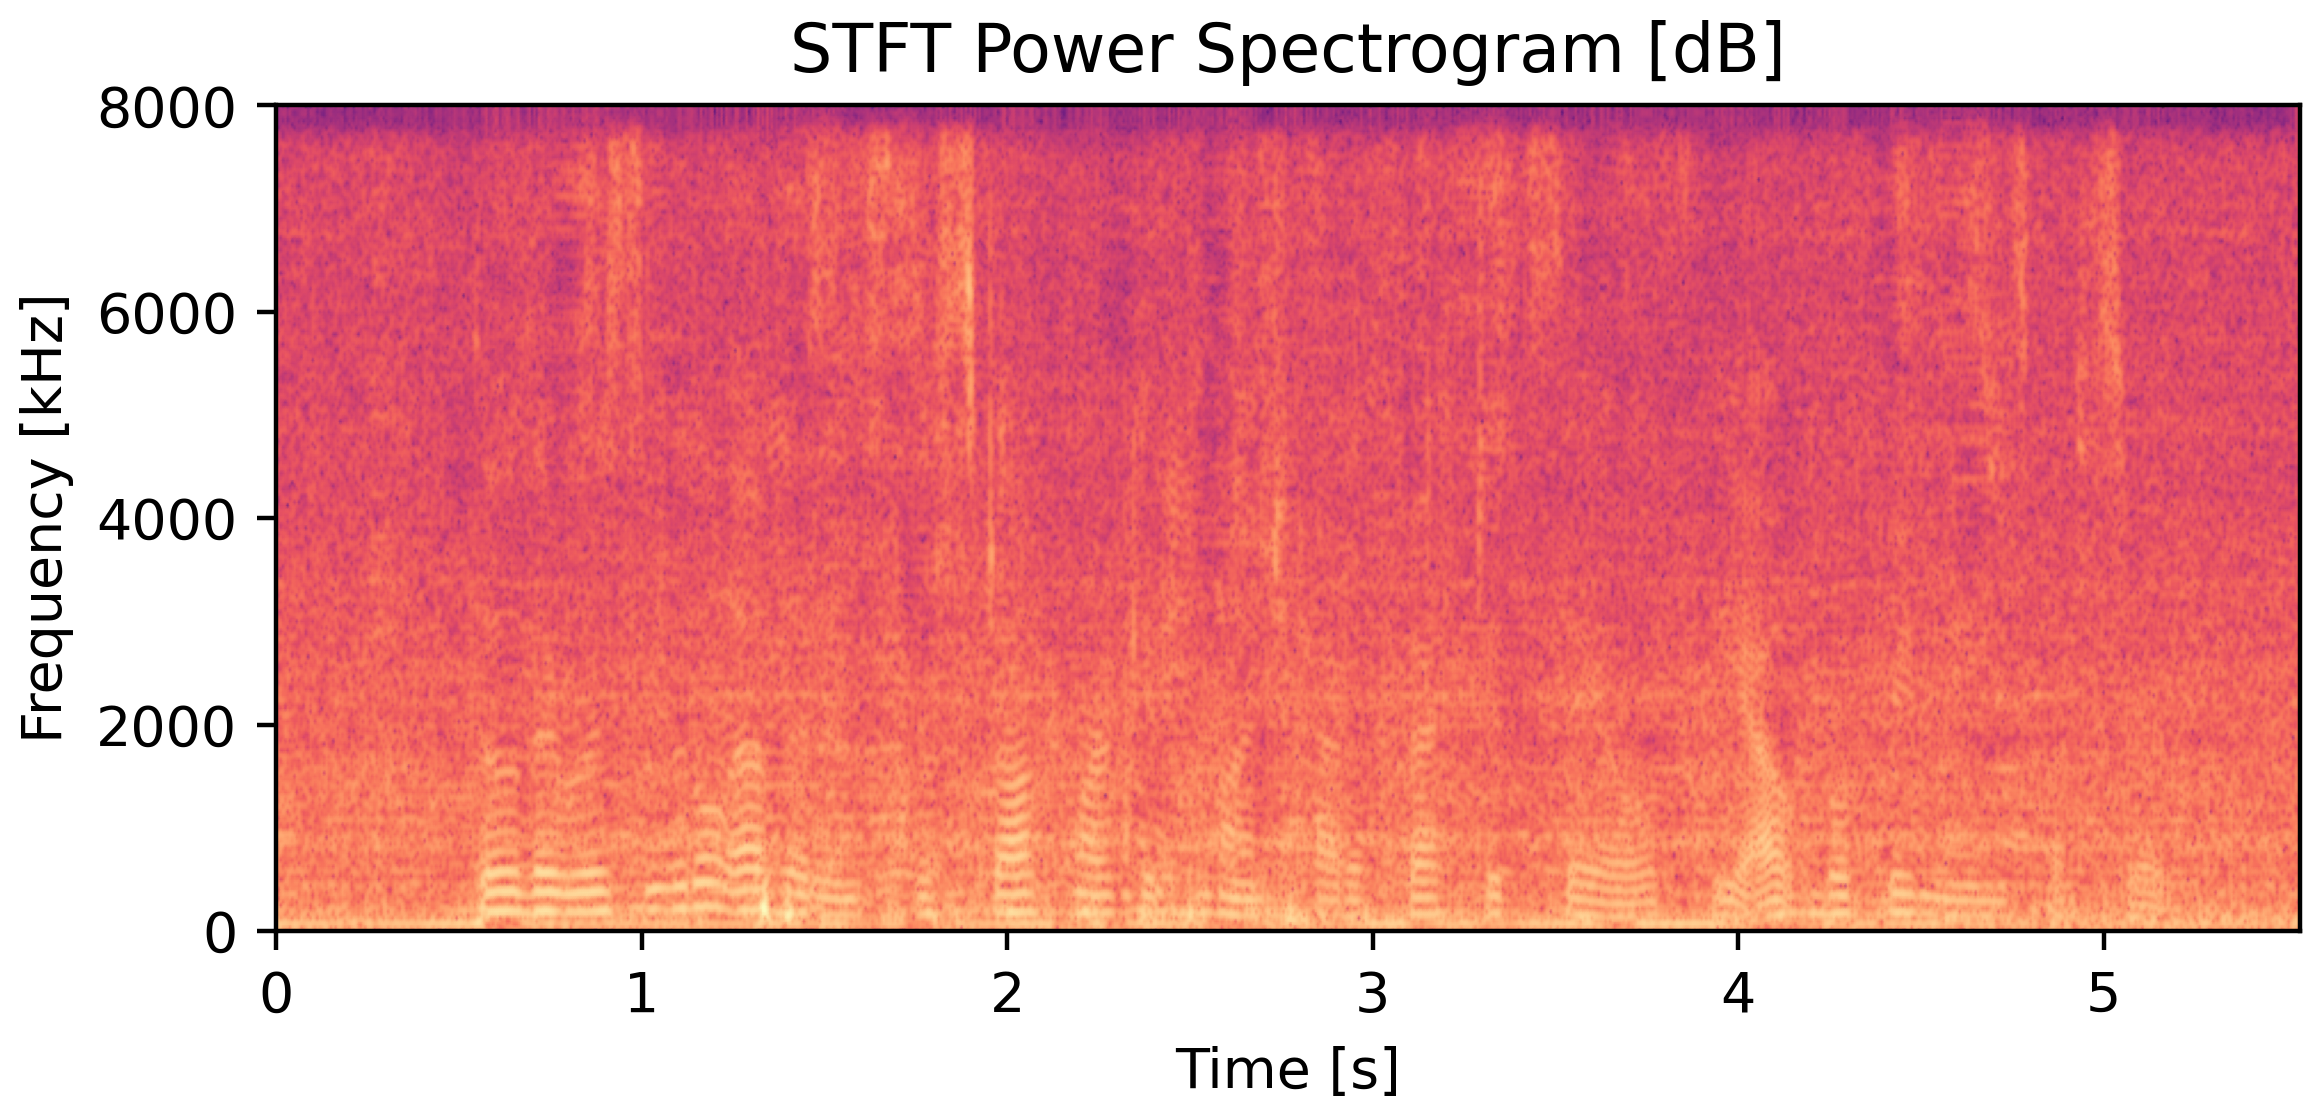
\includegraphics[width=\linewidth]{Features/images/noisy_specgram}
    \caption{Noisy mixture spectrogram}\label{fig:noisy_specgram}
\end{figure}
\begin{figure}[H]
    \centering
    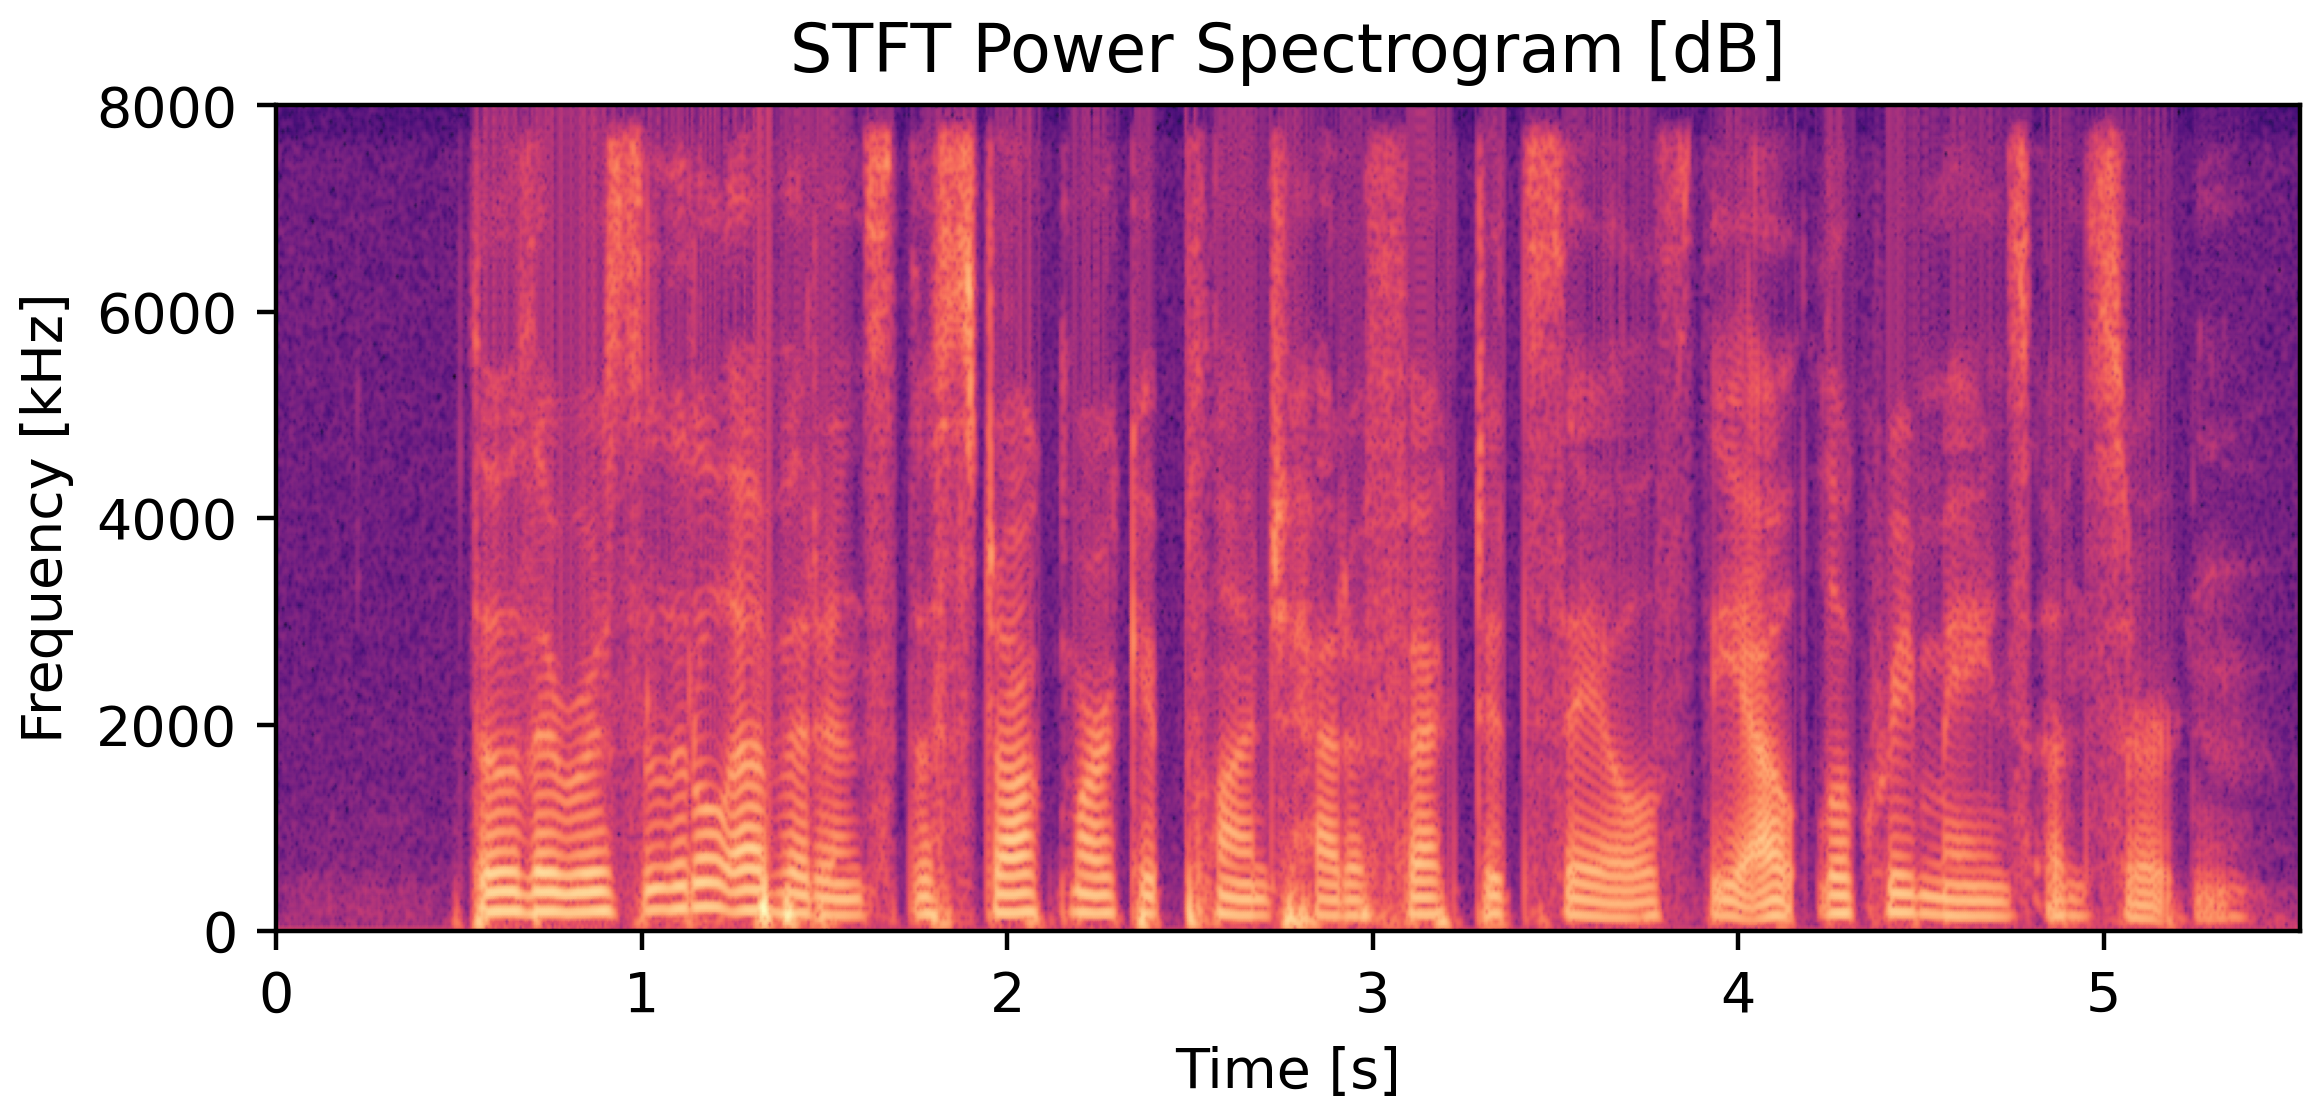
\includegraphics[width=\linewidth]{Features/images/clean_specgram}
    \caption{Reference clean speech spectrogram}\label{fig:clean_specgram}
\end{figure}

Examination of the T-F units provides a 
possibility to classify an entire unit
or parts of a unit 
as a speech-centric bin or, on the contrary, 
as interference (mainly noise). 
Based on this classification, 
appropriate weights are associated with each segment bin.
In that way, speech elements can be extracted 
by separating of the classified speech 
out of the mixture, or alternatively, 
the attenuation of non-speech elements 
in certain activity areas 
along the length of the audio signal.
In general, the association of weights for classifying different
elements in a signal is called T-F masking. 
This process of T-F masking takes a 
significant role in CASA and BSS applications, 
and in recent years, they proved to be 
very useful in E2E-ASR systems.

Additional use of T-F masking 
is to tie it as input to a beamformer that
in turn, filters interferences based 
on the classification received 
by the masking operation.

\section{IBM --- Ideal Binary Mask}
Assuming that a voice activity detection algorithm
can separate speech from noise effectively,
the IBM technique is based on power differences.
Whenever the speech's power 
spectral density (PSD) is higher 
than any of the interferences PSD, 
the speech is masked binarily to ``1''.
\begin{align}\label{eq:ibm_mask}
    \mathbf{M}_{s}(j\omega, t) & = 
        \begin{cases}
            1, & if\;|\mathbf{S}(t,j\omega)|^2 - |\mathbf{N}(t,j\omega)|^2 > \epsilon \\
            0, & otherwise
        \end{cases}
\end{align}
Where \(\epsilon\) marks a changeable threshold value 
for the speech activity detection over the noise.

Equation~\ref{eq:ibm_mask} indicates that as a result of 
applying the IBM masks, the speech and interference separated
sources become complementary in such a way that
\[\mathbf{M}_{n} = 1 - \mathbf{M}_{s} \] and thus:
\begin{align}
    y(t) &= \begin{cases}
        \hat{x_{s}}, &if\;\;\mathbf{M}_{s} = 1 \\
        \hat{x_{n}}, &if\;\;\mathbf{M}_{s} = 0
    \end{cases}
\end{align}

\section{IRM --- Ideal Ratio Mask}
% \begin{align}
%     \mathrm{IRM}(f;t) = \left( \frac{ || }{  } \right)
% \end{align}
Unlike IBM, where hard decisions in terms of 
boolean values are made,
that is, marking speech or noise 
elements with ``true'' or ``false'', the Ideal Ratio Mask (IRM) provides a soft decision
mechanism with values in the range of \([0,1]\)\cite{Jiang2018RobustBF}.
The IRMs at any T-F unit of the clean speech and noise artifacts,
\(\mathbf{M}_{s}(j\omega, t)\) and \(\mathbf{M}_{n}(j\omega, t)\),
are given in 
Equations\;\ref{eq:irm_speech} and \ref{eq:irm_noise}, respectively.

\begin{align}
    \label{eq:irm_speech}\mathbf{M}_{s}(j\omega, t) & = {\left( \frac{|\mathbf{S}(t,j\omega)|^2}{|\mathbf{S}(t,j\omega)|^2 + |\mathbf{N}(t,j\omega)|^2} \right)}^{\beta} \\
    \label{eq:irm_noise}\mathbf{M}_{n}(j\omega, t) & = {\left( \frac{|\mathbf{N}(t,j\omega)|^2}{|\mathbf{S}(t,j\omega)|^2 + |\mathbf{N}(t,j\omega)|^2} \right)}^{\beta}
\end{align}
 
Where \(\beta \) is a tunable parameter that 
controls the strength of the mask estimations. 
A value of 0.5 is used 
for a fair trade-off between speech and noise mask estimations.
%
\begin{align}
    \mathbf{M}_{s}(j\omega, t) & = \sqrt{\left( \frac{|\mathbf{S}(t,j\omega)|^2}{|\mathbf{S}(t,j\omega)|^2 + |\mathbf{N}(t,j\omega)|^2} \right)} \\
    \mathbf{M}_{n}(j\omega, t) & \approx 1 - \mathbf{M}_{s}
\end{align}

\begin{figure}[H]
    \centering
    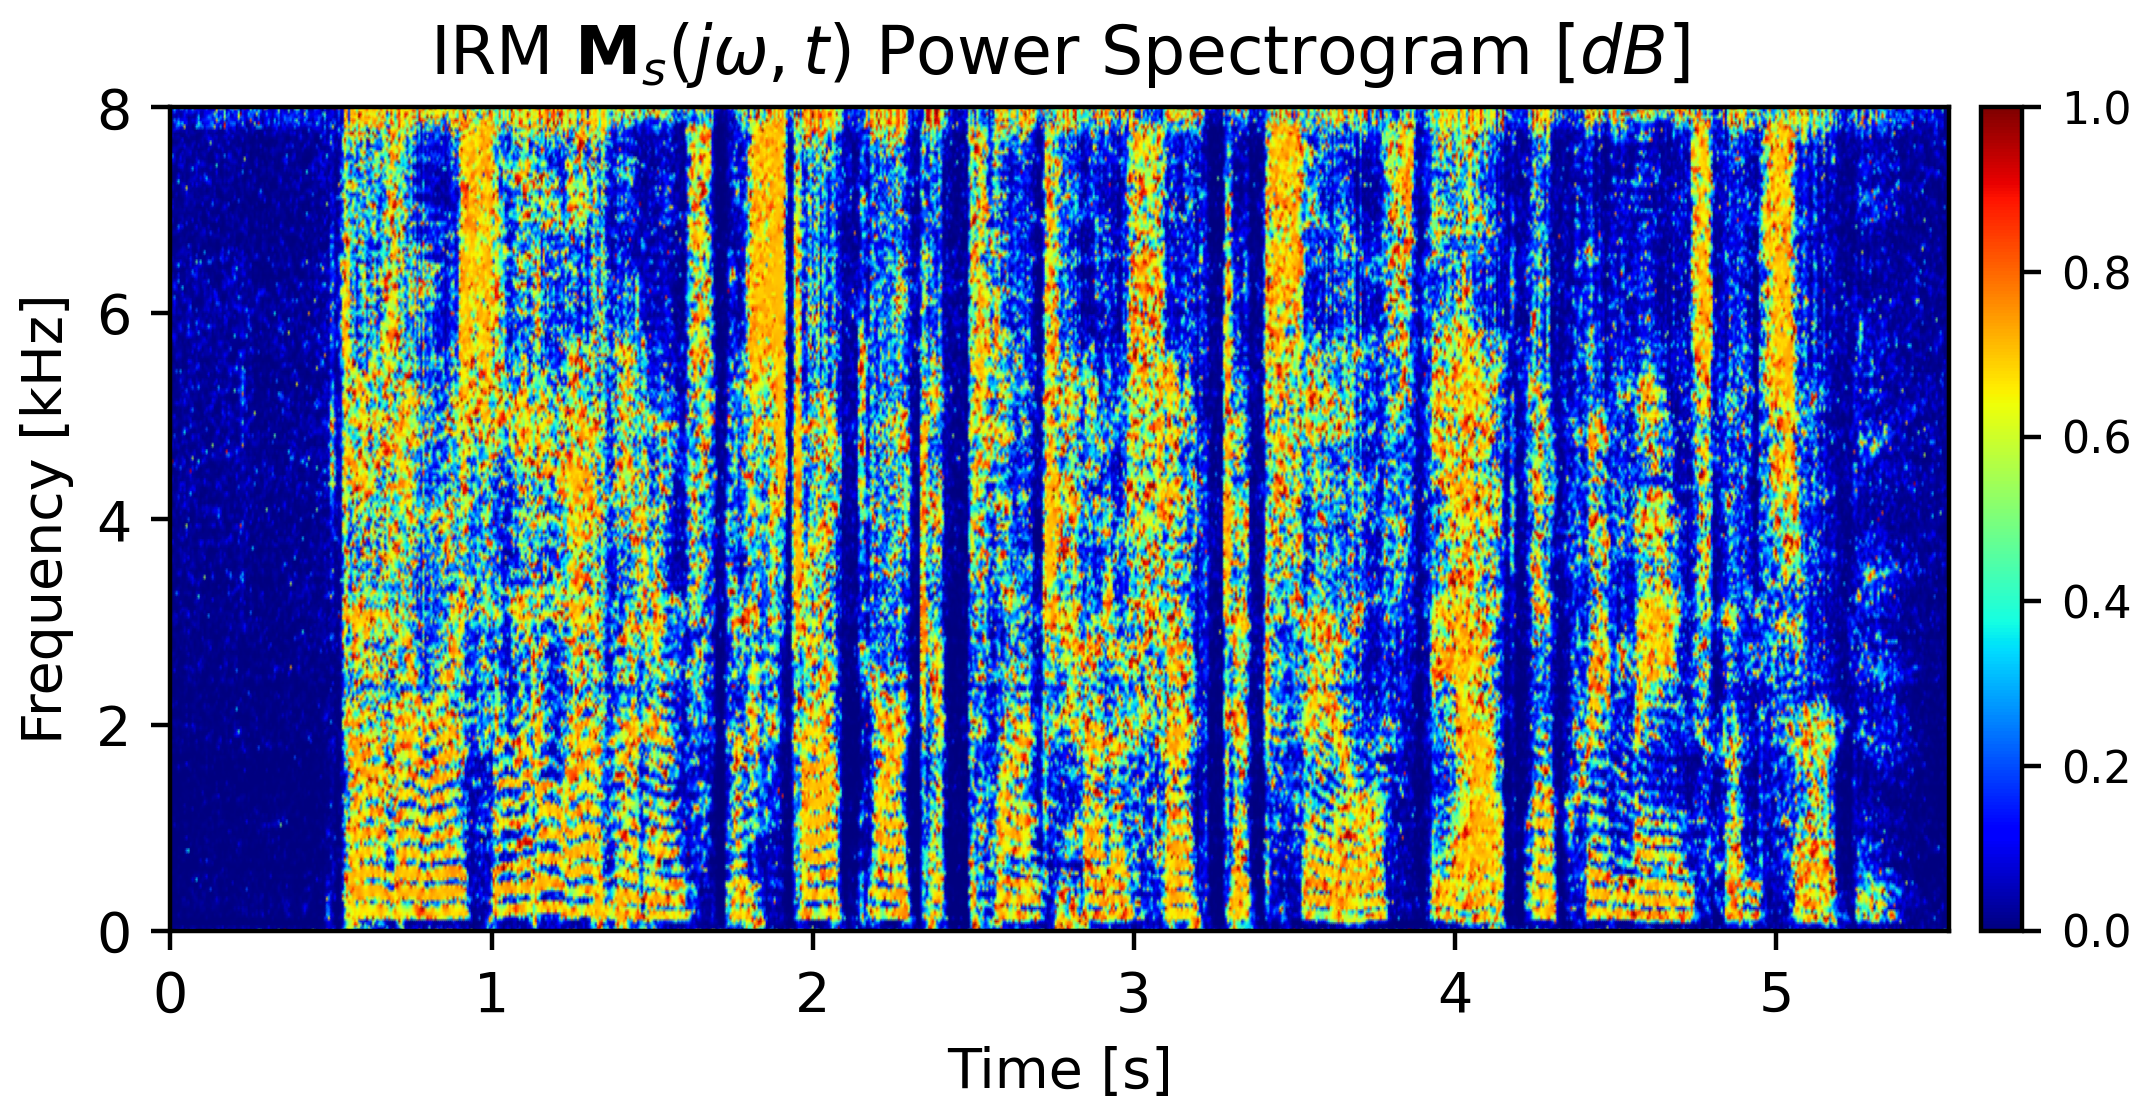
\includegraphics[width=\linewidth]{Features/images/irm_mask}
    \caption{IRM Speech Mask \(\mathbf{M}_{s}(j\omega, t)\)}\label{fig:irm_mask}
\end{figure}
\begin{figure}[H]
    \centering
    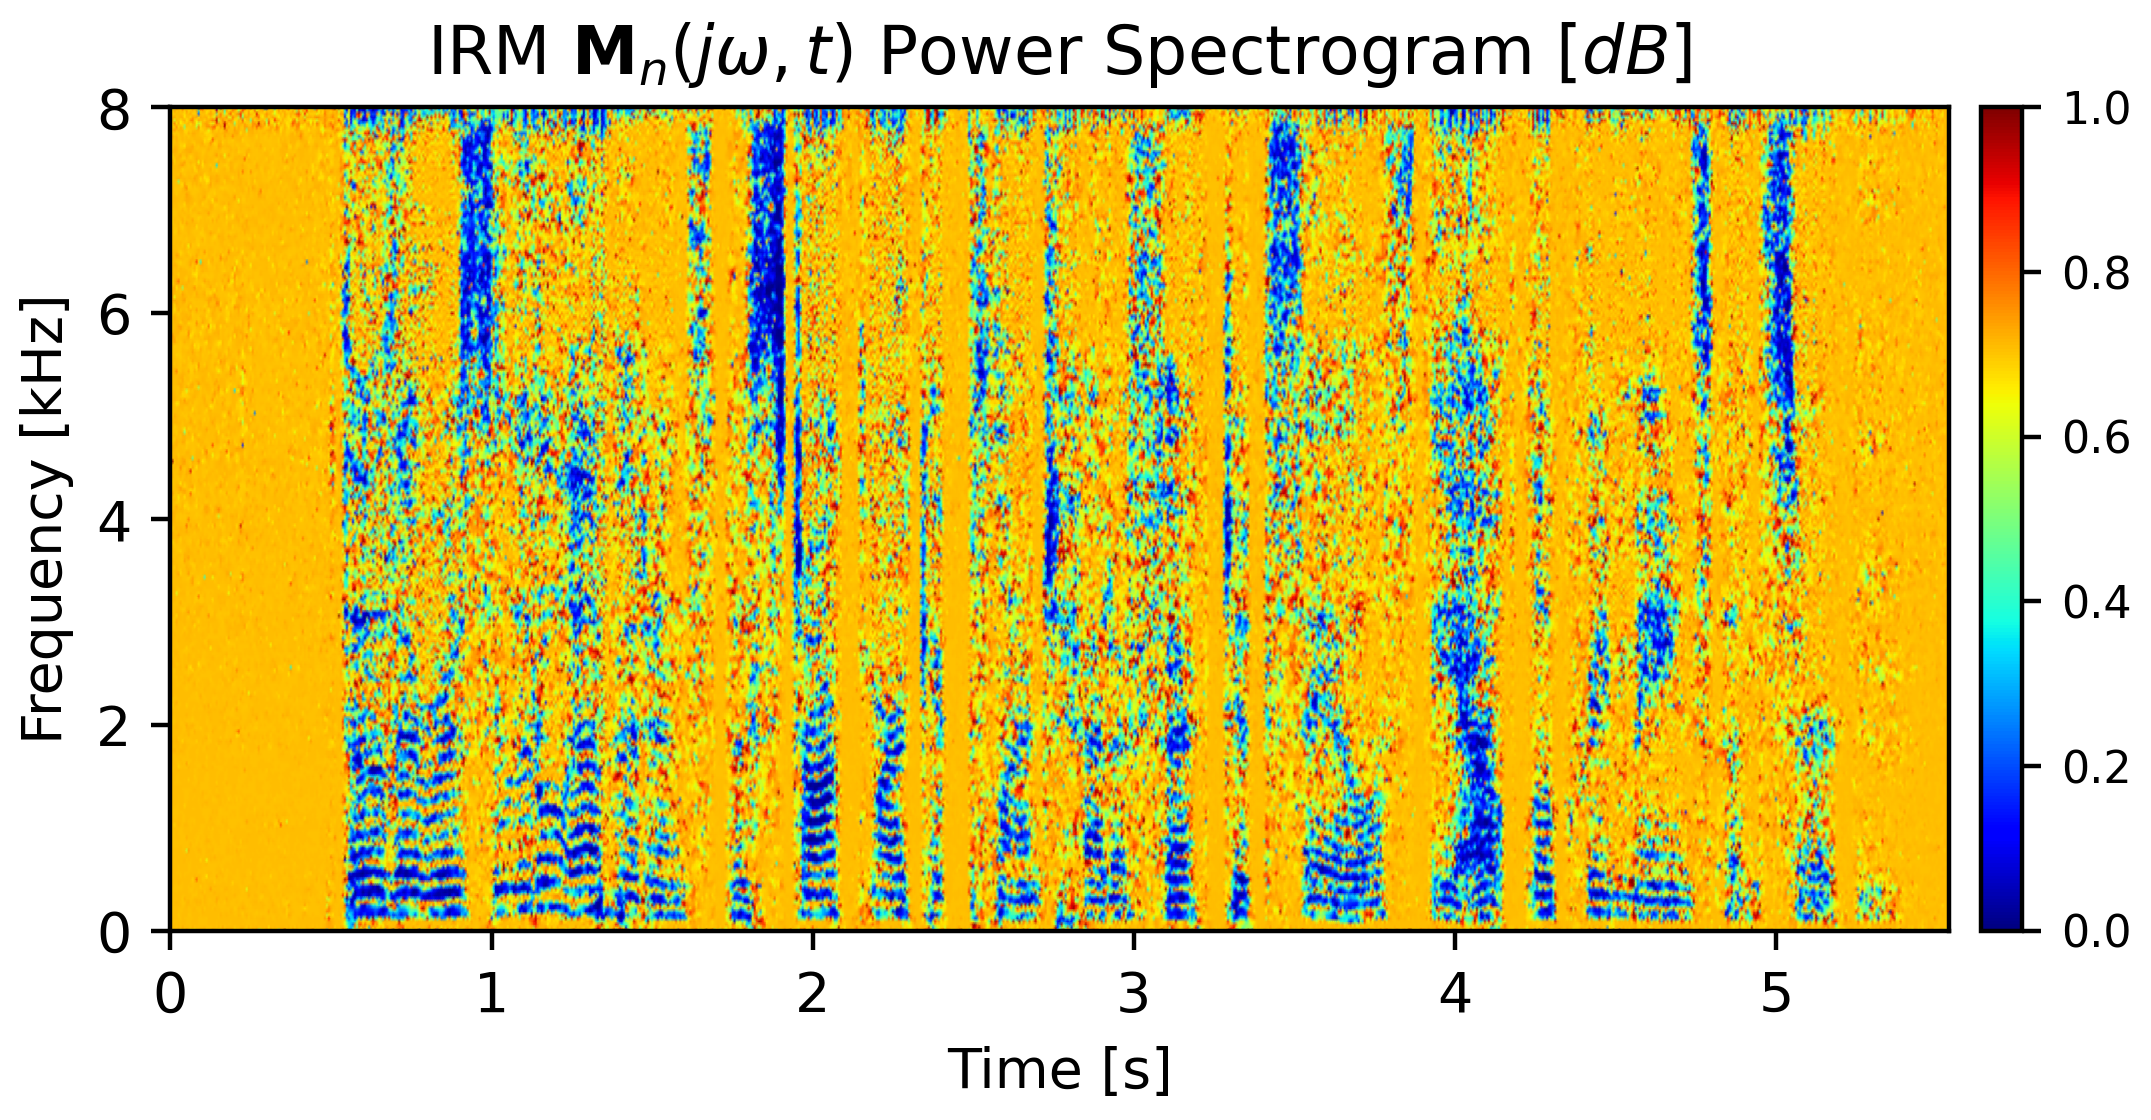
\includegraphics[width=\linewidth]{Features/images/irm_mask_noise}
    \caption{IRM Noise Mask \(\mathbf{M}_{n}(j\omega, t)\)}\label{fig:irm_mask_noise}
\end{figure}

%
Thus, the covariance matrices are extracted by:
\begin{align}
    \mathbf{R}_{NN}(j\omega) & = \frac{1}{\sum\limits_{t=1}^{T}\mathbf{M}_{n_{(jw, t)}}}\sum_{t=1}^{T}\mathbf{M}_{n_{(jw, t)}}|\mathbf{R}_{x_{(jw, t)}}|^2\\
    \mathbf{R}_{SS}(j\omega) & = \frac{1}{\sum\limits_{t=1}^{T}\mathbf{M}_{s_{(jw, t)}}}\sum_{t=1}^{T}\mathbf{M}_{s_{(jw, t)}}|\mathbf{R}_{x_{(jw, t)}}|^2
\end{align}

\subsection{Masks Estimations}
The IRM masks, \(\mathbf{M}_{s}(j\omega, t)\), \(\mathbf{M}_{n}(j\omega, t)\)
given in Equations\;\ref{eq:irm_speech}, \ref{eq:irm_noise} are bounded
in the range of [0, 1]. 
Since both the speech and noise masks are bounded in that range, it is easier
to use a Sigmoid activation function
as the output layer, 
thus ensuring the output indeed remains in this range.

A simple neural network of six to eight fully-connected (FC) layers,
as seen in Figure\;\ref{fig:irm_dnn}, is proposed for
classifying the input features to the desired IRM masks.
The network's input features are the MFCCs of the microphone-array.
Each input signal is framed into \(25ms\) lasting frames with a
hopping length of \(6.25ms\). With a sampling frequency of \(16KHz\), 
the framing settings are 400 samples per frame and 
a total of 300 overlapping samples. 

A BLSTM (Bidirectional Long Short-Term Memory)
layer is placed as the first block in the network,
giving weight to the temporal context as well.
In that way, three additional adjacent feature maps 
are concatenated from both sides of the currently 
processed T-F unit feature map.
The BLSTM is then followed 
by several fully connected (FC) layers 
holding in between the ReLU activation functions.

\begin{figure}[H]
    \centering
    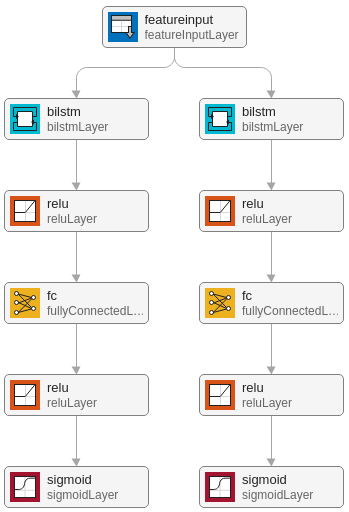
\includegraphics[width=0.95\linewidth]{Features/images/irm_dnn}
    \caption{IRM estimation DNN blocks diagram}\label{fig:irm_dnn}
\end{figure}

Production of both the speech and noise estimations co-occurs. 
Consequently, the cost function should 
consider the two masks in the 
minimization process of the error term.
To that end, the cost function is defined as:
\begin{align}
    \ell(\mathbf{\widehat{M}}_{j\omega, t},\;\mathbf{M}_{j\omega, t}) & = 
        \frac{1}{2N}\sum_{j\omega, t}
        \left[ 
            \beta\!\left( 
                \mathbf{\widehat{M}}^{(s)}_{j\omega, t} - 
                \mathbf{M}^{(s)}_{j\omega, t} 
            \right)^{2} 
            + \left( 1- \beta \right)\!
            \left(
                \mathbf{\widehat{M}}^{(n)}_{j\omega, t} - 
                \mathbf{M}^{(n)}_{j\omega, t} 
            \right)^{2} 
        \right]
\end{align}
Here, \(\beta\) denotes the weighing factor.
For a fair and evenly consideration between the masks, \(\beta \)
is set to 0.5.

The proposed IRM estimation network blocks diagram is shown in 
Figure\;\ref{fig:irm_nn}.

\begin{figure}[H]
    \centering
    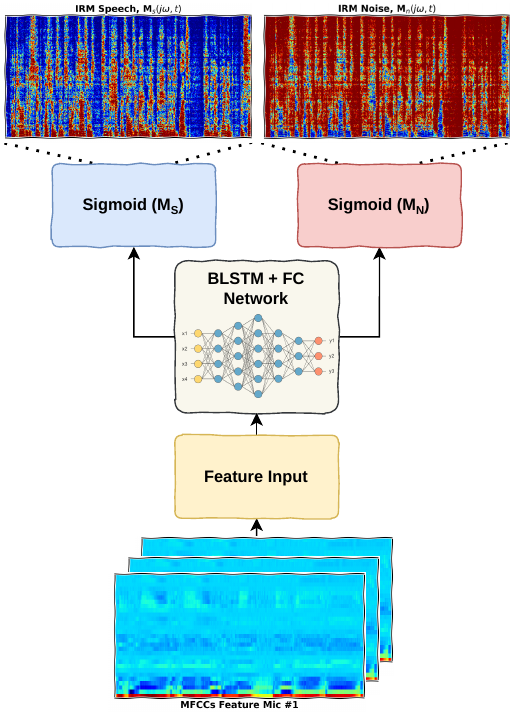
\includegraphics[width=0.75\linewidth]{Beamformers/images/irm_nn}
    \caption{Proposed DNN for IRM T-F masking estimations}\label{fig:irm_nn}
\end{figure}


\begin{figure}[H]
    \centering
    \subfloat[\label{irm_s_ref}]{%
       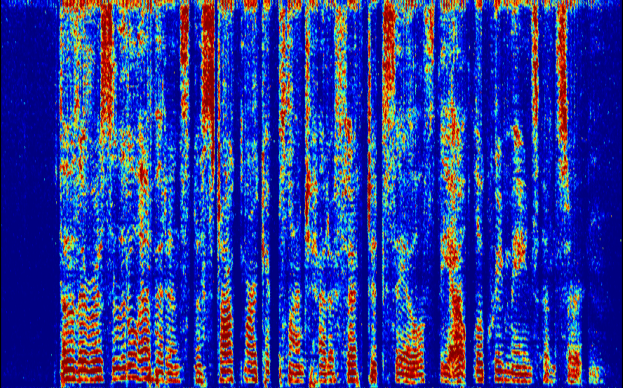
\includegraphics[width=0.45\linewidth]{Beamformers/images/irm_s_ref}}
    \hspace{0.1cm}
    \subfloat[\label{irm_s_nn}]{%
        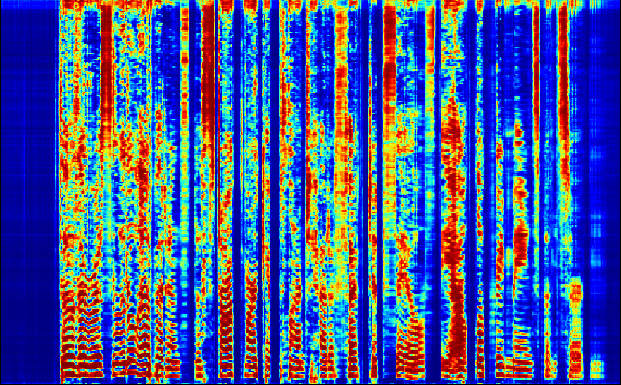
\includegraphics[width=0.45\linewidth]{Beamformers/images/irm_s_nn}}
    \vspace{-0.35cm}
    \subfloat[\label{irm_n_ref}]{%
        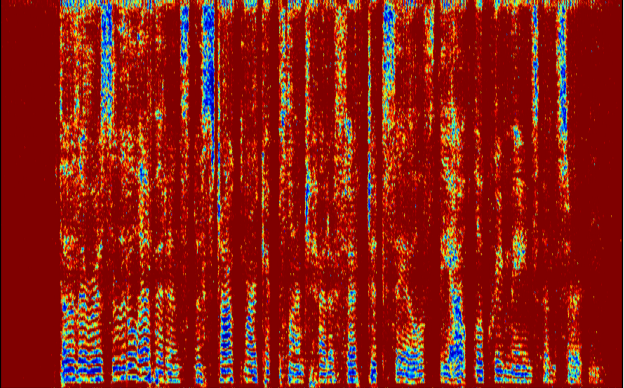
\includegraphics[width=0.45\linewidth]{Beamformers/images/irm_n_ref}}
    \hspace{0.1cm}
    \subfloat[\label{irm_n_nn}]{%
        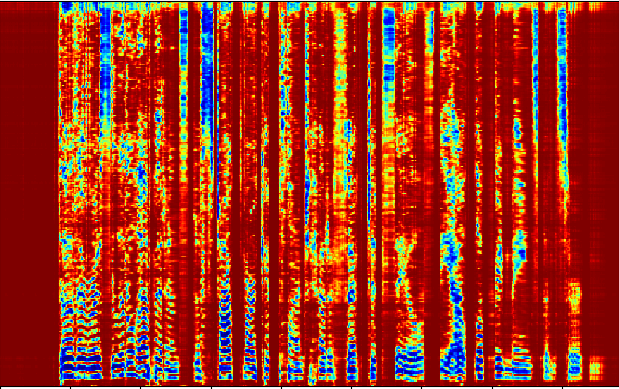
\includegraphics[width=0.45\linewidth]{Beamformers/images/irm_n_nn}}
        \caption{(a) and (b) are the ``IRM'' 
        reference vs. estimation masks of the speech.
        \(\mathbf{\widehat{M}}^{(s)}_{j\omega, t}\), \(\mathbf{M}^{(s)}_{j\omega, t}\);\;\;
        (c) and (d) are the ``IRM'' reference vs. estimation masks 
        of the noise \(\mathbf{\widehat{M}}^{(n)}_{j\omega, t}\), \(\mathbf{M}^{(n)}_{j\omega, t}\).}\label{fig:irm_ref_s_n} 
\end{figure}


\subsection{Measurements}
\subsubsection{SNR}
\begin{figure}[H]
    \centering
    \subfloat[\label{irm_enh_snr}]{%
       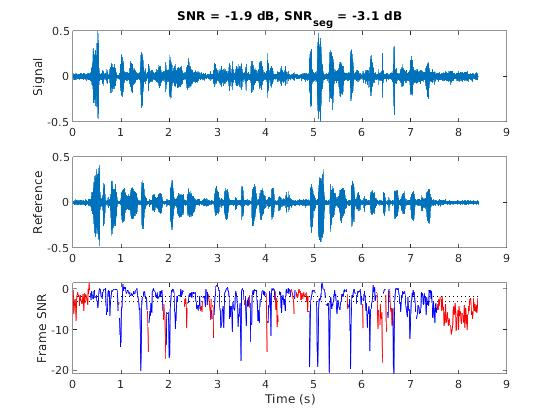
\includegraphics[width=0.5\linewidth]{Features/images/irm_enh_snr}}
    % \hspace{0.1cm}
    \subfloat[\label{irm_noisy_snr}]{%
        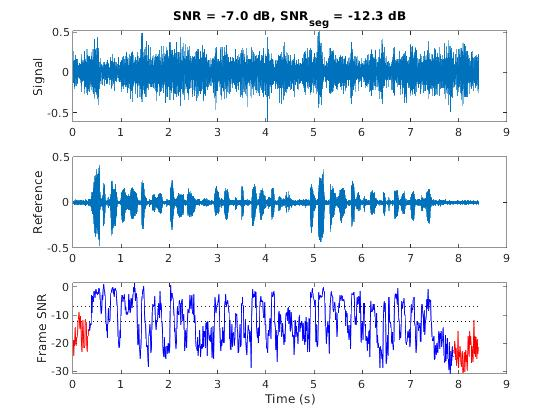
\includegraphics[width=0.5\linewidth]{Features/images/irm_noisy_snr}}
    \caption{(a) ``IRM'' enhanced SNR \& Segmental-SNR degradation
        with respect to the clean reference speech;\;\;
        (b) The SNR \& Segmental-SNR ratios between the
        clean reference speech and the noisy mixture.}\label{fig:irm_enh_noisy_snr} 
\end{figure}

Figure\;\ref{fig:irm_enh_noisy_snr} shows two measurements of the SNR \&
Segmental-SNR metrics for two subject signals, 
an ``IRM'' enhanced beamformed
version of the noisy mixture and the noisy mixture itself
with respect to the clean reference speech.
The overall improvements in SNR and Segmental-SNR 
are the ratios between the enhanced beamformed signal
and the noisy mixture. Thus, from Figure\;\ref{fig:irm_enh_noisy_snr}
the accumulated improvement in SNR is:
\[|SNR_{noisy}| - |SNR_{enh}| = 5.1725\;[dB]\]
Likewise, the improvement in Segmental-SNR is \(9.2675\;[dB]\).
It is important to note that the enhanced beamformed signal
does not align in time with the clean speech reference. 
In a worst-case scenario, we measured a delay of \(-0.0014\;[s]\),
which equals approximately \(22\) samples. 
A perfectly aligned comparison considers being more 
accurate, but since the frame lengths' (400 samples)
are much larger than the worst measured delay, 
the impact of this time misalignment is less acute.
The Segmental-SNR calculation involves 
a VAD (voice activity detection) algorithm
for dropping segments where the detected speech activity is negligible.
These dropped segments are red colored in Figure\;\ref{fig:irm_enh_noisy_snr}.

\begin{figure}[H]
    \centering
    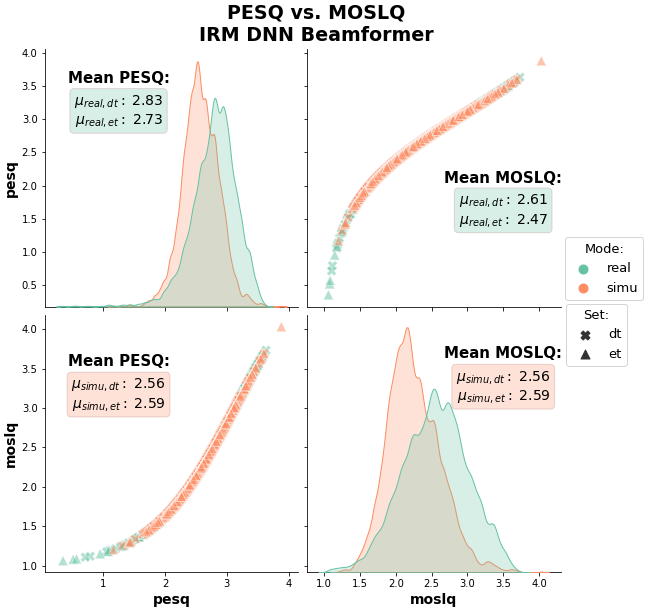
\includegraphics[width=\linewidth]{Experiments/images/irm_pesq_mosq}
    \caption{IRM beamformer PESQ vs. MOSLQ}\label{fig:irm_pesq_mosq}
\end{figure}

In Figure\;\ref{fig:irm_pesq_mosq} presented the ``PESQ'' and ``MOSLQ'' 
metrics for the IRM beamformer. The results are shown in a pair-plot
diagram, where the correlations between each pair of metrics are plotted.
On the diagonal, the distributions of the measured values are shown.
On top of the plots also shown are the mean values for both 
the ``PESQ'' and ``MOSLQ'' under the test cases of the real and 
simulation datasets from the ``CHiME4'' dataset. ``et'' stands for
the evaluation subset and ``dt'' marks the development subset.
More details about the datasets are provided in Chapter\;\ref{ch:datasets}.

A strong correlation between the ``PESQ'' and ``MOSLQ'' is seen in the
plot, and this behavior is both understandable and desirable since
the ``MOSLQ'' metric is based on the ``PESQ'' measurement.

Another pair-plot for the SNR, ``Segmental-SNR'', ``SI-SNR'' and ``STOI''
metrics is shown in Figure\;\ref{fig:irm_snr_stoi}.
The ``simulation'' subset yields better results in terms of
performance. It is important to note that faulty microphones
in the ``real'' subset are dropped prior to taking the measurements.
Nevertheless, the ambient noise absorbed is characterized by
a real scenario and a non-artificial room impulse response. On the other hand,
the ``simulation'' subset is composed of a recording taken in a relatively
clean environment (recording booth) and an artificial mixture of
the recorded background noises.

Because the SNR and Segmental-SNR are measured as the improvement
compared to the noisy mixture, 
and since the background noises are truncated 
to match the booth recorded speech for the ``simulation'' subset, 
the results for those metrics are more sparsely distributed 
compared to the ``real'' subset measurements. 
With the ``SI-SNR'', 
the measurements are taken regardless of the noisy mixture. 
Hence, the ``simulation'' results are far better 
and more spatially dense 
in contrast to the ``real'' subset ``SI-SNR'' results.

Likewise, in the same manner, 
the ``STOI'' is measured regardless of the noisy mixture
but relatively to the clean speech. 
Therefore, the ``simulation'' 
subset distribution is narrower with lower variance.

% The results are summarized in Table\;\ref{tbl:irm_snr_stoi},
% side by side with the ideal masks and the improvement ratios.

\begin{figure}[H]
    \centering
    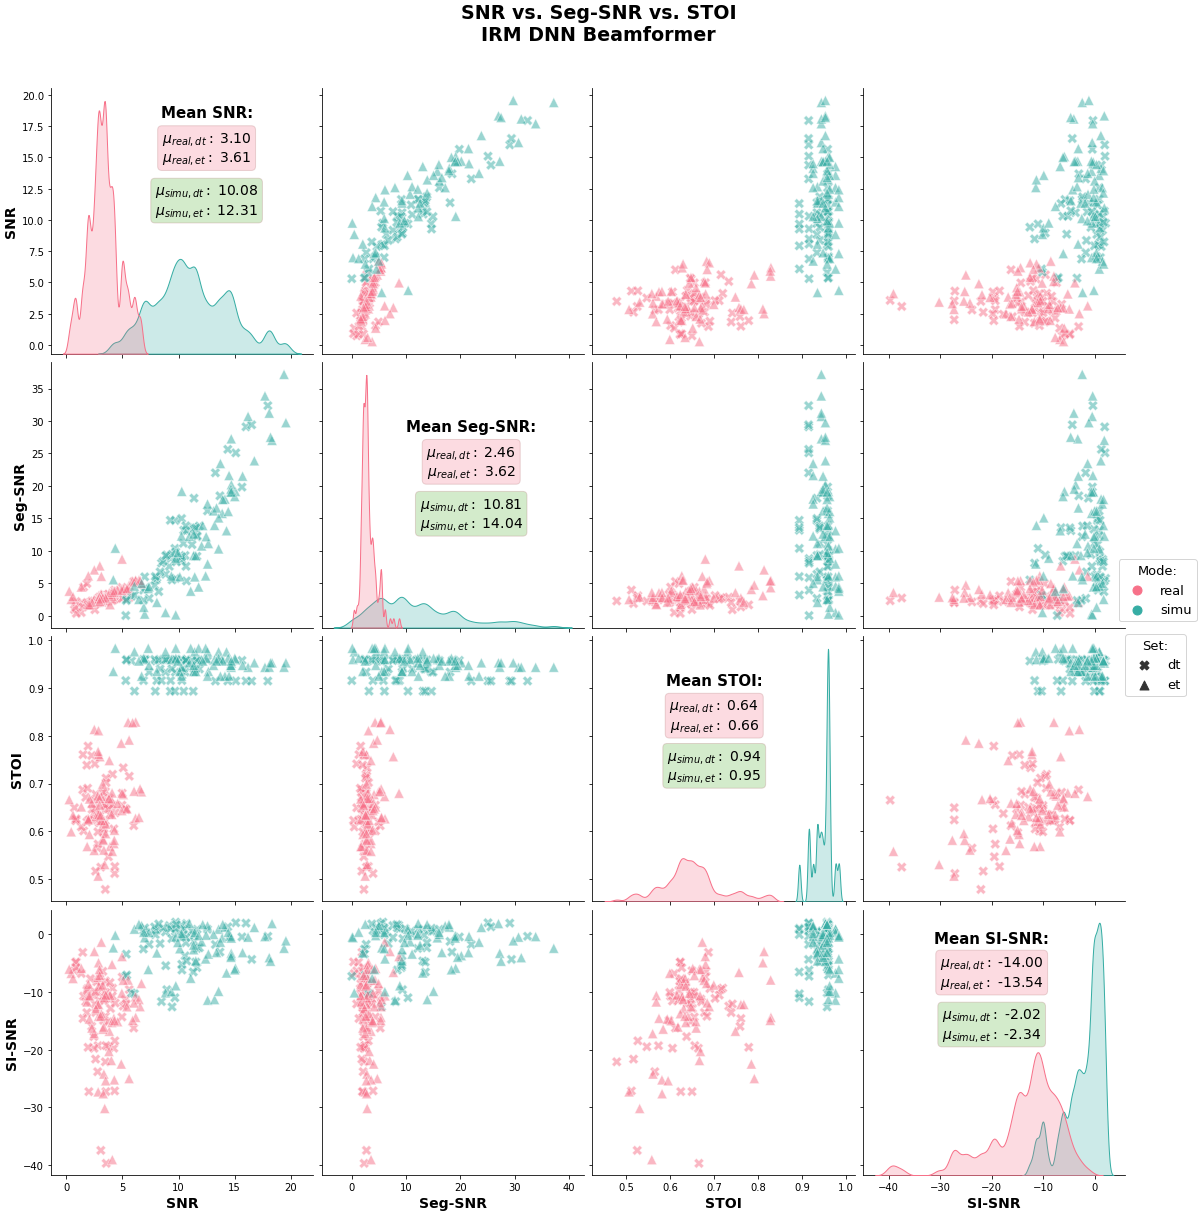
\includegraphics[width=\linewidth]{Features/images/irm_snr_stoi}
    \caption{IRM beamformer SNR vs. Segmental-SNR vs. STOI vs. SI-SNR}\label{fig:irm_snr_stoi}
\end{figure}

In order to evaluate the generalization of the prediction model,
the DNN estimations are compared to the ideal mask enhancement.
In Figure\;\ref{fig:irm_ideal_snr}, shown is the measurements of 
the SNR and ``Segmental-SNR'' for an ideal IRM mask.
SNR measurement.

\begin{figure}[H]
    \centering
    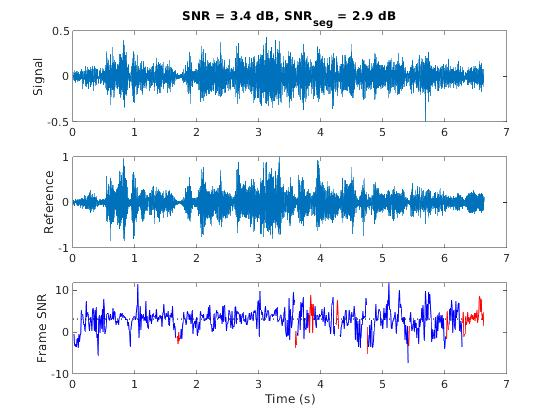
\includegraphics[width=\linewidth]{Features/images/irm_ideal_snr}
    \caption{Ideal IRM beamformer enhancement SNR \& Segmental-SNR.}\label{fig:irm_ideal_snr}
\end{figure}



\section{cIRM --- Complex Ideal Ratio Mask}\label{ssec:cirm}
Both IBM and IRM utilize the noise and speech magnitudes only
while completely neglecting the phase arguments.
The outcome of the STFT operation is a complex pair
representation of each T-F unit. Recent studies
showed the importance of 
the phase element in 
speech seperation\cite{7364200,Xia2017UsingOR}.

In that manner, further extension of the IRM mask 
to include the imaginary part 
altogether with the magnitudes forms the cIRM. 
Thus, instead of having a magnitude only based mask matrix, a complex
pair of masking matrices that make use of the phase element too is given.

The mixture \(y(t)\) after being processed by
the STFT operation can be described as a complex sum
whether in polar coordinates as seen in Equation\ref{eq:ystft_polar}
or in the general form as in Equation\ref{eq:ystft_general}.
\begin{align}\label{eq:ystft_polar}
    \mathbf{Y}(j\omega, t)  & = \mathcal{STFT} \{ y(t) \} := \mathbf{Y}_{j\omega, t} \nonumber \\
                            & = |\mathbf{A}_{_{\mathbf{Y}}}|\cos(\bm{\theta}_{_{\mathbf{Y}}}) 
                            + j|\mathbf{A}_{_{\mathbf{Y}}}|\sin(\bm{\theta}_{_{\mathbf{Y}}}) \\
\label{eq:ystft_general}      & = \mathbf{Y}_{r} + j\mathbf{Y}_{i}
\end{align}

The real and imaginary parts can be summarized as:
\begin{align}
    \mathbf{Y}_{r} & := \mathfrak{R}_{_{\mathfrak{C}}} \{\mathbf{Y}_{j\omega, t}\} 
                            = |\mathbf{A}_{_{\mathbf{Y}}}|\cos(\bm{\theta}_{_{\mathbf{Y}}})  \\
    \mathbf{Y}_{i} & := \mathfrak{T}_{_{\mathfrak{M}}} \{\mathbf{Y}_{j\omega, t}\} 
                            = |\mathbf{A}_{_{\mathbf{Y}}}|\sin(\bm{\theta}_{_{\mathbf{Y}}})
\end{align}
Extraction of the magnitude and phase from the complex representation 
is accomplished by the following set of 
Equations\ref{eq:complex_mag},\ref{eq:complex_phase}:
\begin{align}\label{eq:complex_mag}
    |\mathbf{A}_{_{\mathbf{Y}}}|    & = \sqrt{ \mathfrak{R}_{_{\mathfrak{C}}} \{\mathbf{Y}_{j\omega, t}\}^{2}
                                            + \mathfrak{T}_{_{\mathfrak{M}}} \{\mathbf{Y}_{j\omega, t}\}^{2} } \\
    \label{eq:complex_phase}\bm{\theta}_{_{\mathbf{Y}}}     & = \tan^{-1} \Bigg\{ \frac{ \mathfrak{T}_{_{\mathfrak{M}}} \{\mathbf{Y}(j\omega, t)\} }
                                            {\mathfrak{R}_{_{\mathfrak{C}}} \{\mathbf{Y}(j\omega, t)\}} \Bigg\}
\end{align}
Rearranging the equations above, 
we can write the cIRM mask's real and 
imaginary parts as:
\begin{align}
    \mathbf{M}_{r} & = \frac{\mathbf{Y}_{r}\mathbf{S}_{r} + \mathbf{Y}_{i}\mathbf{S}_{i}}
                            { \mathbf{Y}_{r}^{2} + \mathbf{Y}_{i}^{2}} \\
    \mathbf{M}_{i} & = \frac{\mathbf{Y}_{r}\mathbf{S}_{i} - \mathbf{Y}_{i}\mathbf{S}_{r}}
                            { \mathbf{Y}_{i}^{2} + \mathbf{S}_{r}^{2}}
\end{align}
Thus, the complex masks for the speech and noise are: 
\begin{align}
    \mathbf{M}^{(s)}_{j\omega, t} & = \mathbf{M}^{(s)}_{r} + j\mathbf{M}^{(s)}_{i} \nonumber \\
            & = \frac{\mathbf{Y}_{r}\mathbf{S}_{r} + \mathbf{Y}_{i}\mathbf{S}_{i}}
            { \mathbf{Y}_{r}^{2} + \mathbf{Y}_{i}^{2}} 
            + j \frac{\mathbf{Y}_{r}\mathbf{S}_{i} - \mathbf{Y}_{i}\mathbf{S}_{r}}
            { \mathbf{Y}_{i}^{2} + \mathbf{S}_{r}^{2}} \label{eq:cirmr_mask} \\
    \mathbf{M}^{(n)}_{j\omega, t} & = \mathbf{M}^{(N)}_{r} + j\mathbf{M}^{(N)}_{i} \nonumber \\
    & = \frac{\mathbf{Y}_{r}\mathbf{N}_{r} + \mathbf{Y}_{i}\mathbf{N}_{i}}
    { \mathbf{Y}_{r}^{2} + \mathbf{Y}_{i}^{2}} 
    + j \frac{\mathbf{Y}_{r}\mathbf{N}_{i} - \mathbf{Y}_{i}\mathbf{N}_{r}}
    { \mathbf{Y}_{i}^{2} + \mathbf{N}_{r}^{2}} \label{eq:cirmi_mask}
\end{align}
Therefore, applying a cIRM T-F masking requires a complex multiplication
for separation as opposed to the more basic IBM and IRM 
where magnitudes multiplications are taken in the real domain only.

The reference compressed cIRM masks are 
shown in Figure\;\ref{fig:cirm_ref_s_n};

\begin{figure}[H]
    \centering
    \subfloat[\label{cIRM_real_mask}]{%
       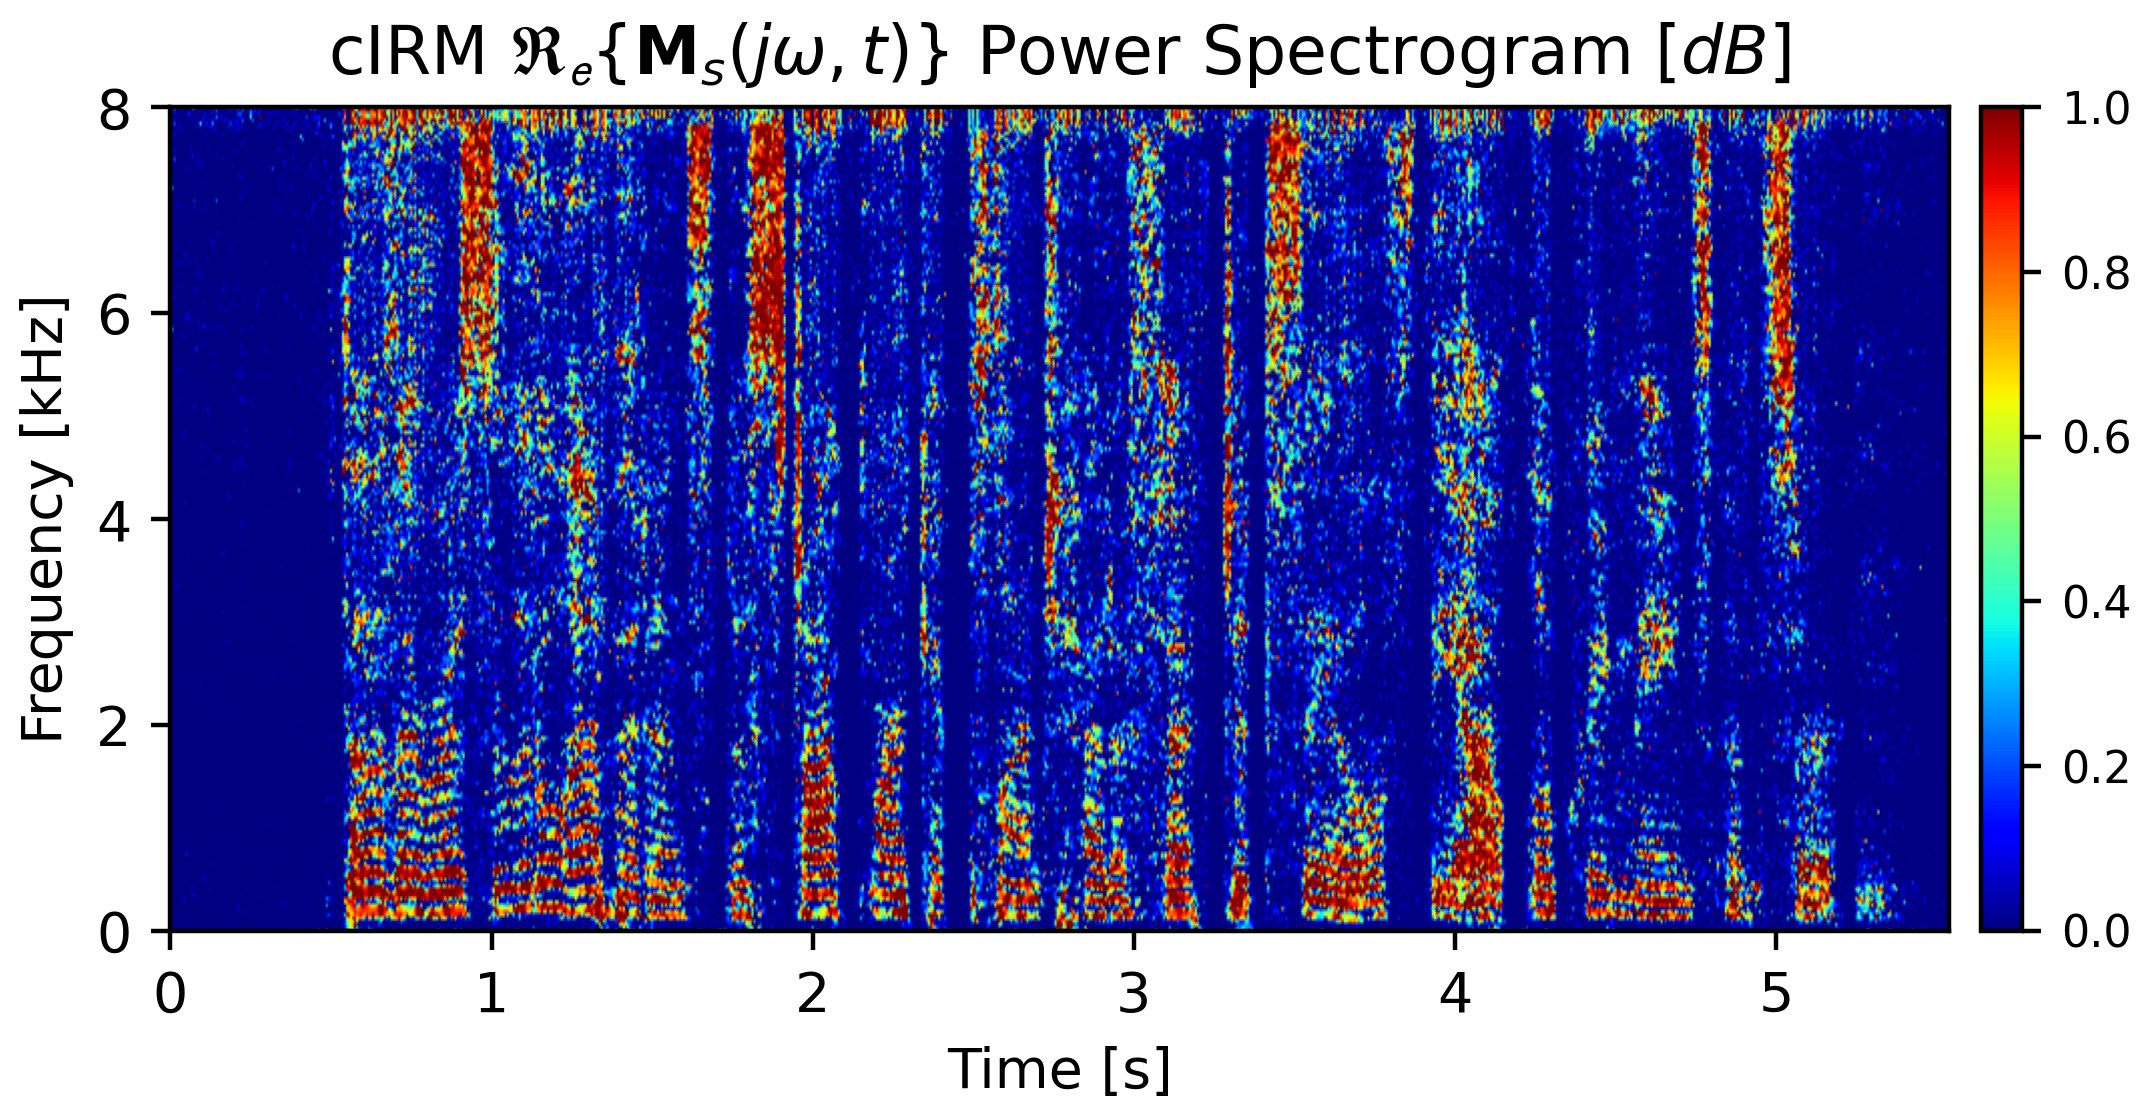
\includegraphics[width=0.45\linewidth]{Features/images/cIRM_real_mask}}
    \subfloat[\label{cIRM_imag_mask}]{%
        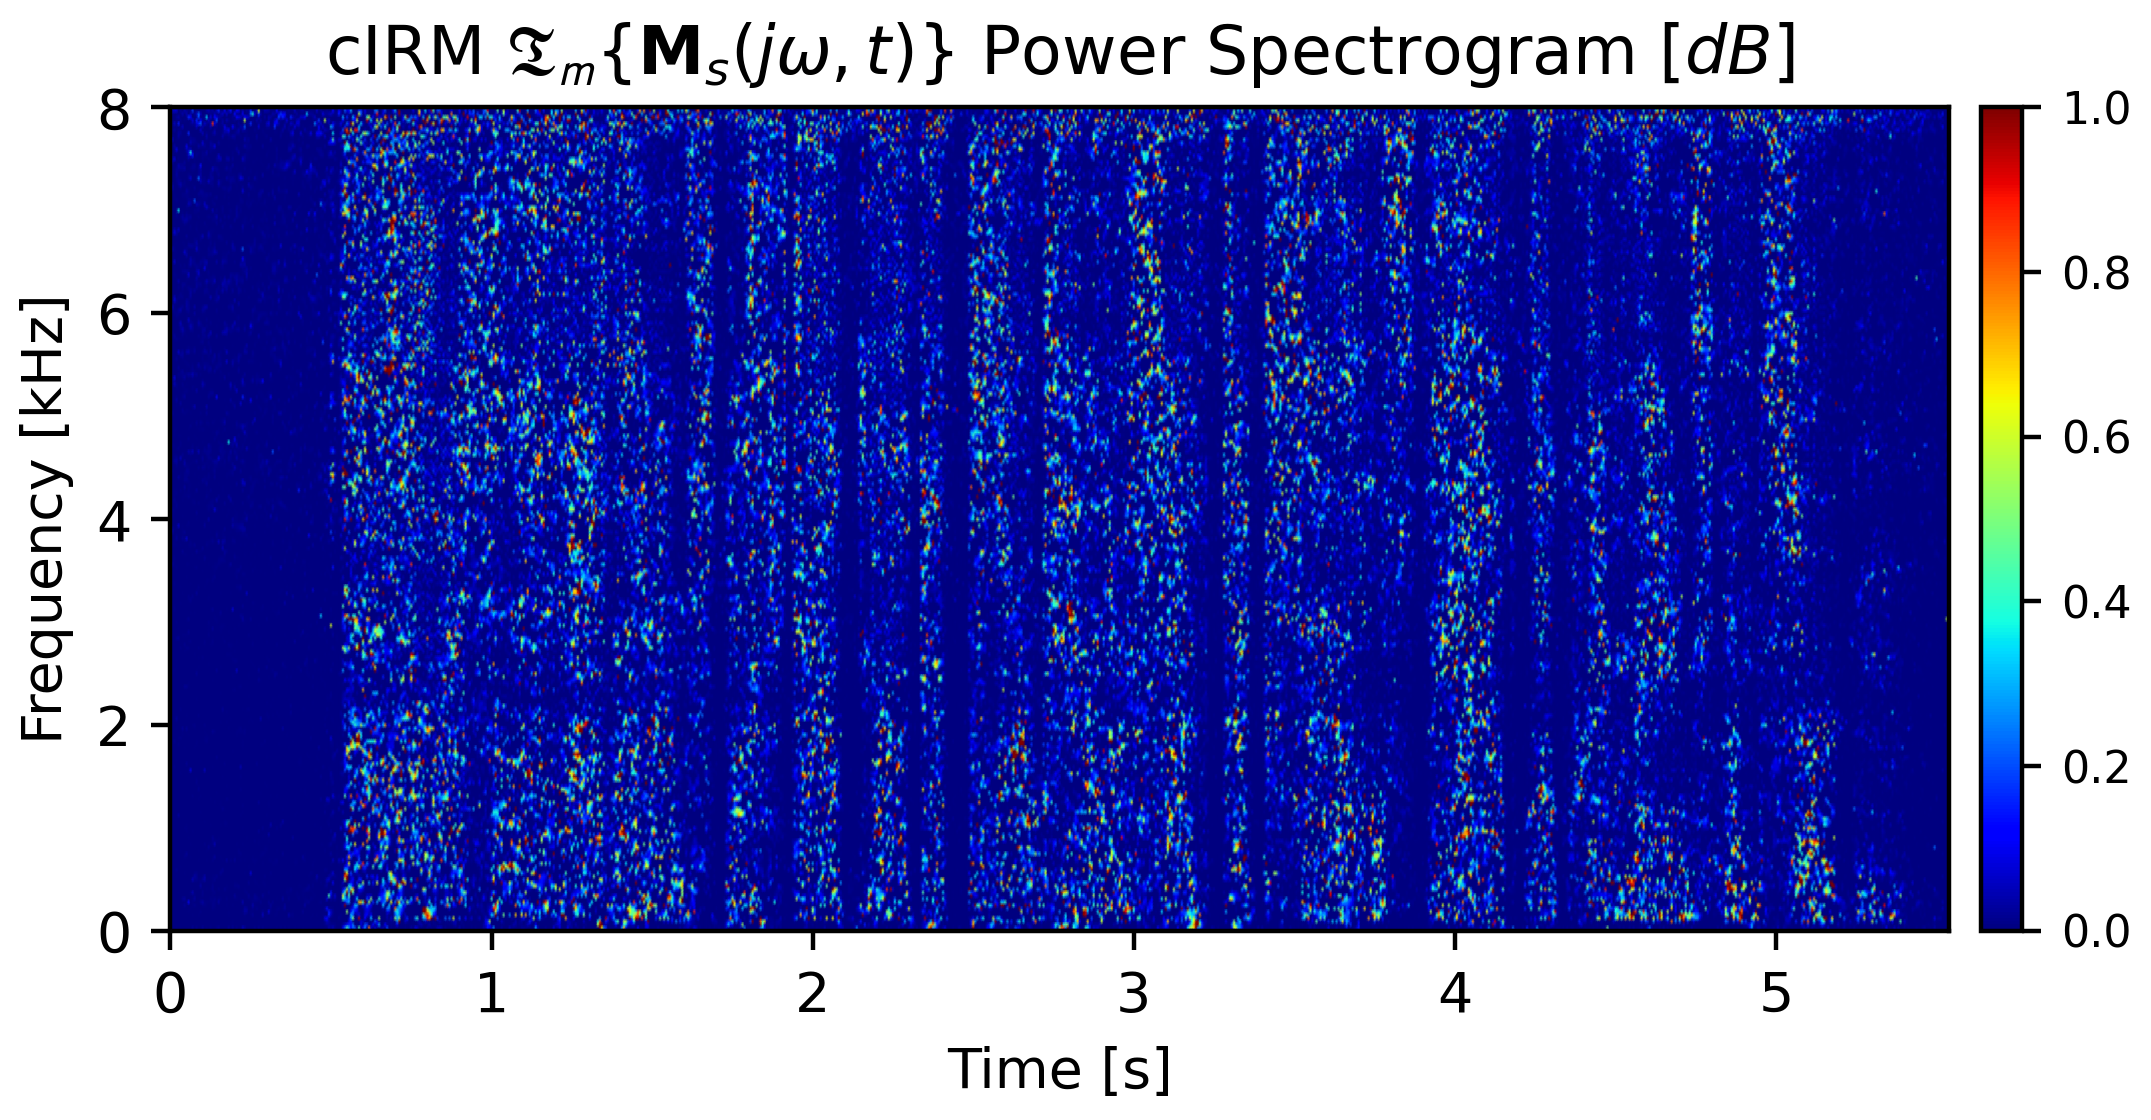
\includegraphics[width=0.45\linewidth]{Features/images/cIRM_imag_mask}}
    \vspace{-0.35cm}
    \subfloat[\label{cIRM_real_noise_mask}]{%
        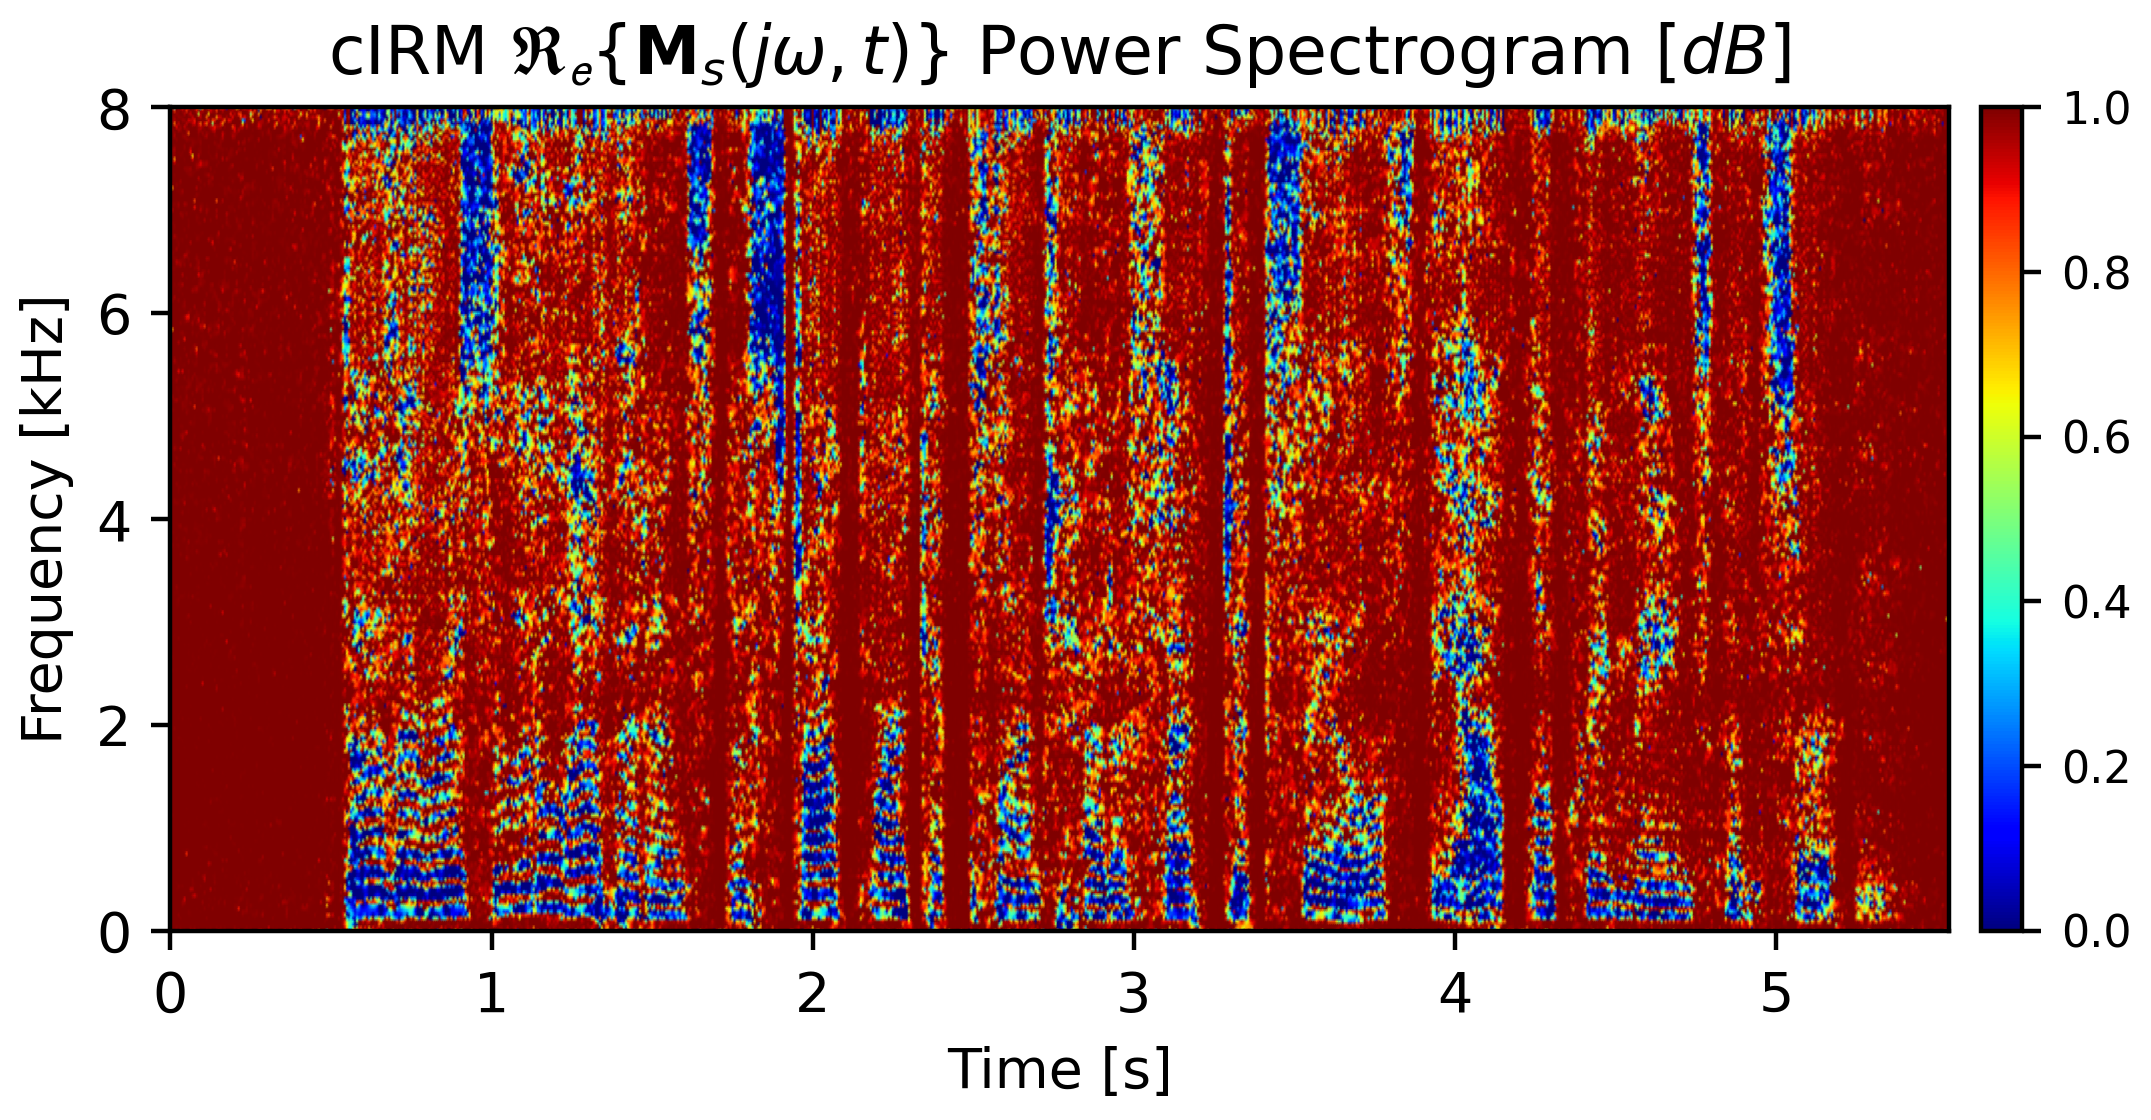
\includegraphics[width=0.45\linewidth]{Features/images/cIRM_real_noise_mask}}
    \subfloat[\label{cIRM_imag_noise_mask}]{%
        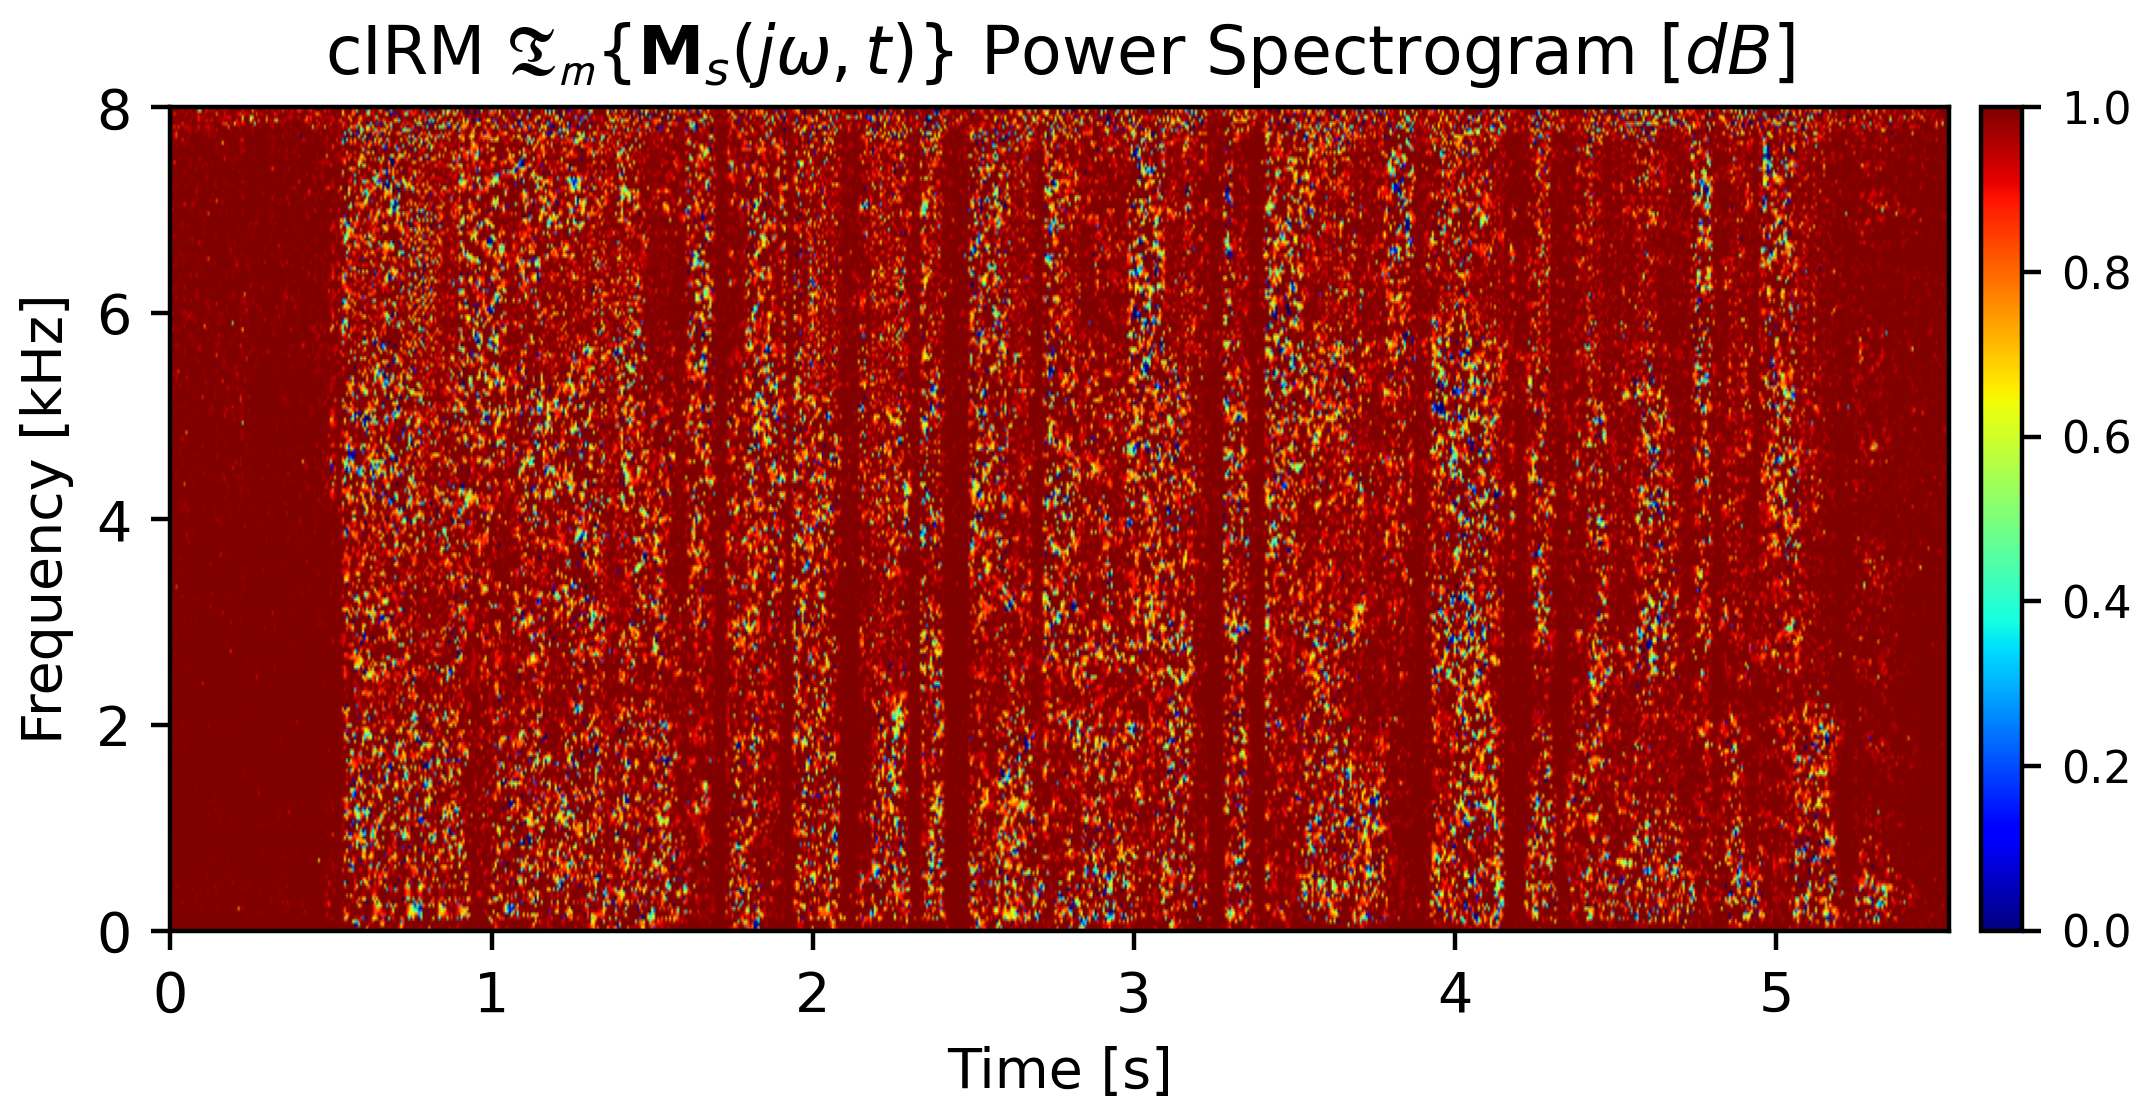
\includegraphics[width=0.45\linewidth]{Features/images/cIRM_imag_noise_mask}}
        \caption{(a) and (b) are the cIRM
        real and imaginary references of the speech 
        \(\mathbf{M}^{(s)}_{r}\), \(\mathbf{M}^{(s)}_{i}\);\;\;
        (c) and (d) are the cIRM real and imaginary references 
        of the noise \(\mathbf{M}^{(n)}_{r}\), \(\mathbf{M}^{(n)}_{i}\).}\label{fig:cirm_ref_s_n} 
\end{figure}

\subsection{Masks Estimations}
In Section~\ref{ssec:cirm}, 
the \(cIRM\) masks are described in 
Equations~\ref{eq:cirmr_mask},~\ref{eq:cirmi_mask}.
In contrast to the \(IRM\) masks which are bounded in the range \([0, 1]\),
the \(cIRM\) masks are unbounded, and have the range \((-\infty, \infty)\).

A neural network cannot train for unbounded values. 
Hence, an alternative presentation to the mask values is needed.
One possibility is to compress the real and imaginary masks
with a hyperbolic tangent as suggested in \cite{7364200}: 
\begin{align}\label{eq:cirm_compress}
    cIRM_{x} &= K \frac{1-e^{-C\cdot M_{x}}}{1+e^{-C\cdot M_{x}}}
\end{align}
Where \(x\) stands for the real or the imaginary parts of the mask.
By applying this compression, the mask values are bounded in
the range \([-K, K]\), while \(C\) controls the steepness.
For that purpose, we replaced the 
simpler IRM DNN sigmoid layers placed at the output 
with linear layers.

Then, the cost function is defined to include both real and imaginary parts
of both the noise and speech masks. 
\begin{align}
    \ell(\mathbf{\widehat{M}}^{(x)}_{j\omega, t},\;\mathbf{M}^{(x)}_{j\omega, t}) & = 
        \frac{1}{2N}\sum_{j\omega, t}
        \left[ 
            \beta\!\left( 
                \mathbf{\widehat{M}}^{(s \in \mathbb{C})}_{j\omega, t} - 
                \mathbf{M}^{(s \in \mathbb{C})}_{j\omega, t} 
            \right)^{2} 
            + \left( 1- \beta \right)\!
            \left(
                \mathbf{\widehat{M}}^{(n \in \mathbb{C})}_{j\omega, t} - 
                \mathbf{M}^{(n \in \mathbb{C})}_{j\omega, t} 
            \right)^{2} 
        \right]
\end{align}

The proposed cIRM estimation network blocks 
diagram is shown in Figure\;\ref{fig:cirm_nn}.

\begin{figure}[H]
    \centering
    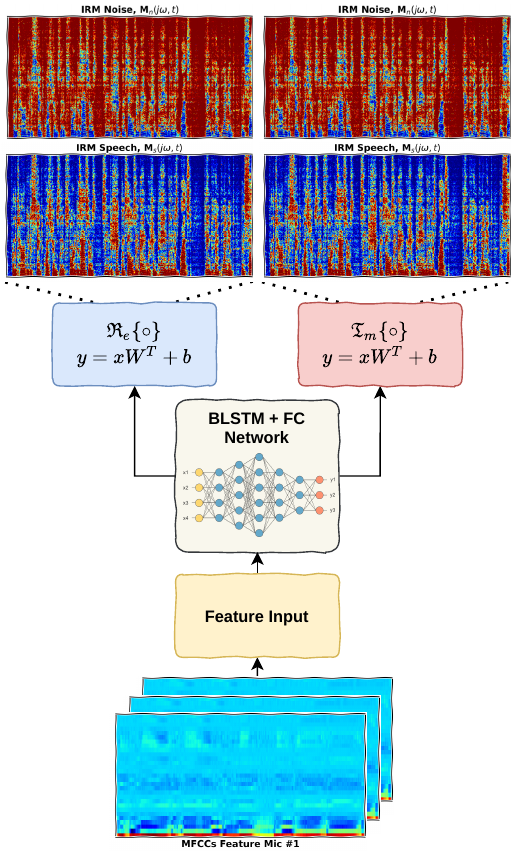
\includegraphics[width=0.75\linewidth]{Beamformers/images/cirm_nn}
    \caption{Proposed DNN for cIRM T-F masking estimations}\label{fig:cirm_nn}
\end{figure}


\begin{figure}[H]
    \centering
    \subfloat[\label{mel_fb_ref}]{%
       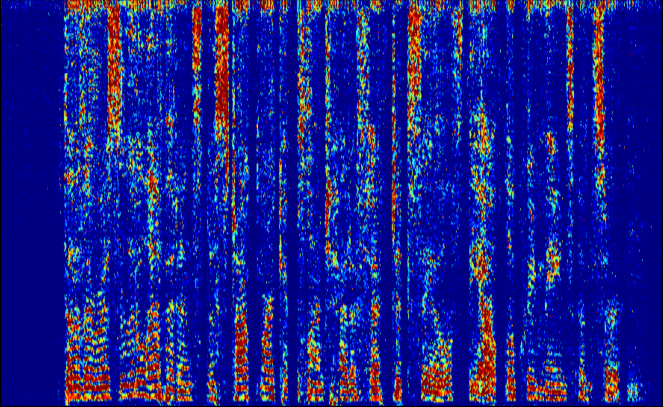
\includegraphics[width=0.45\linewidth]{Beamformers/images/cirm_r_s_ref}}
    \hspace{0.1cm}
    \subfloat[\label{mel_fbfcc_ref}]{%
        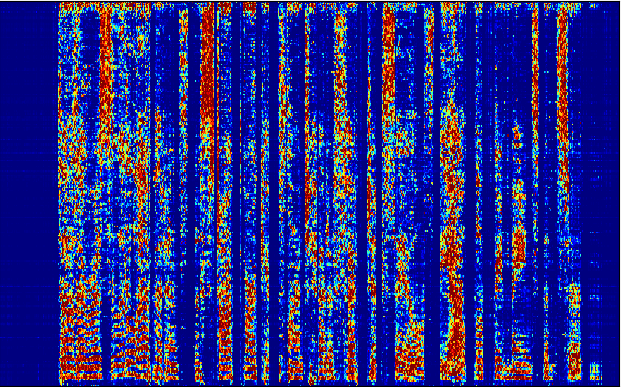
\includegraphics[width=0.444\linewidth]{Beamformers/images/cirm_r_s_nn}}
    \caption{(a) Reference cIRM
        real speech mask \(\mathbf{M}^{(s)}_{r}\);\;\;
        (b) The estimated cIRM
        real speech \(\mathbf{\widehat{M}}^{(s)}_{r}\).}\label{fig:cirm_nn_vs_ref} 
\end{figure}

Figure\;\ref{fig:cirm_nn_vs_ref} shows the reference real speech cIRM mask
compared to the estimated real speech mask predicted by the DNN model.
Looking at the figure, one can conclude that the model generalized correctly
as the estimated mask resembles the reference to a great extent.
Compared to the ``IRM'' DNN performance, the cIRM model 
with a compression in the range of \([-10, 10]\) performs better.

\subsection{Measurements}
Due to the complexity of the cIRM DNN model, 
it did not generalize properly for the evaluation dataset
with a number of epochs settings set to 50.
The results hence, are not accurate as a reference nor for comparison,
unless a retraining process is initialized with a sufficient number of epochs
to let the model generalize.

Due to the uncertainty of the impact the low number of epochs have
on the model performance, and the lack of time for a re-evaluation of the
DNN mask estimation, we decide to skip the results and 
to drop the cIRM measurements.

% \begin{figure}[H]
%     \centering
%     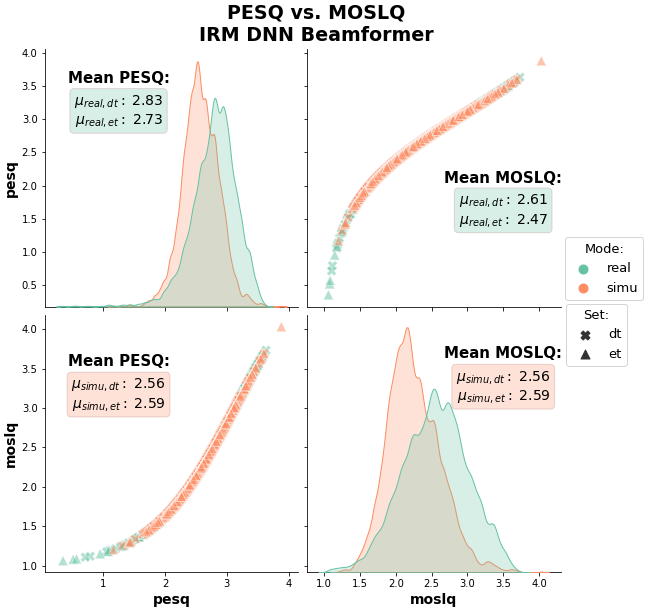
\includegraphics[width=\linewidth]{Experiments/images/irm_pesq_mosq}
%     \caption{IRM beamformer PESQ vs. MOSLQ}\label{fig:irm_pesq_mosq}
% \end{figure}

\section{PSM --- Phase Sensitive Mask}
The PSM T-F masking makes use of the magnitude ratios and phase differences
rather than requiring a complex multiplication.
In that way, the multiplication is taken in the real domain only,
while utilizing the phase contribution directly.

\begin{figure}[H]
    \centering
    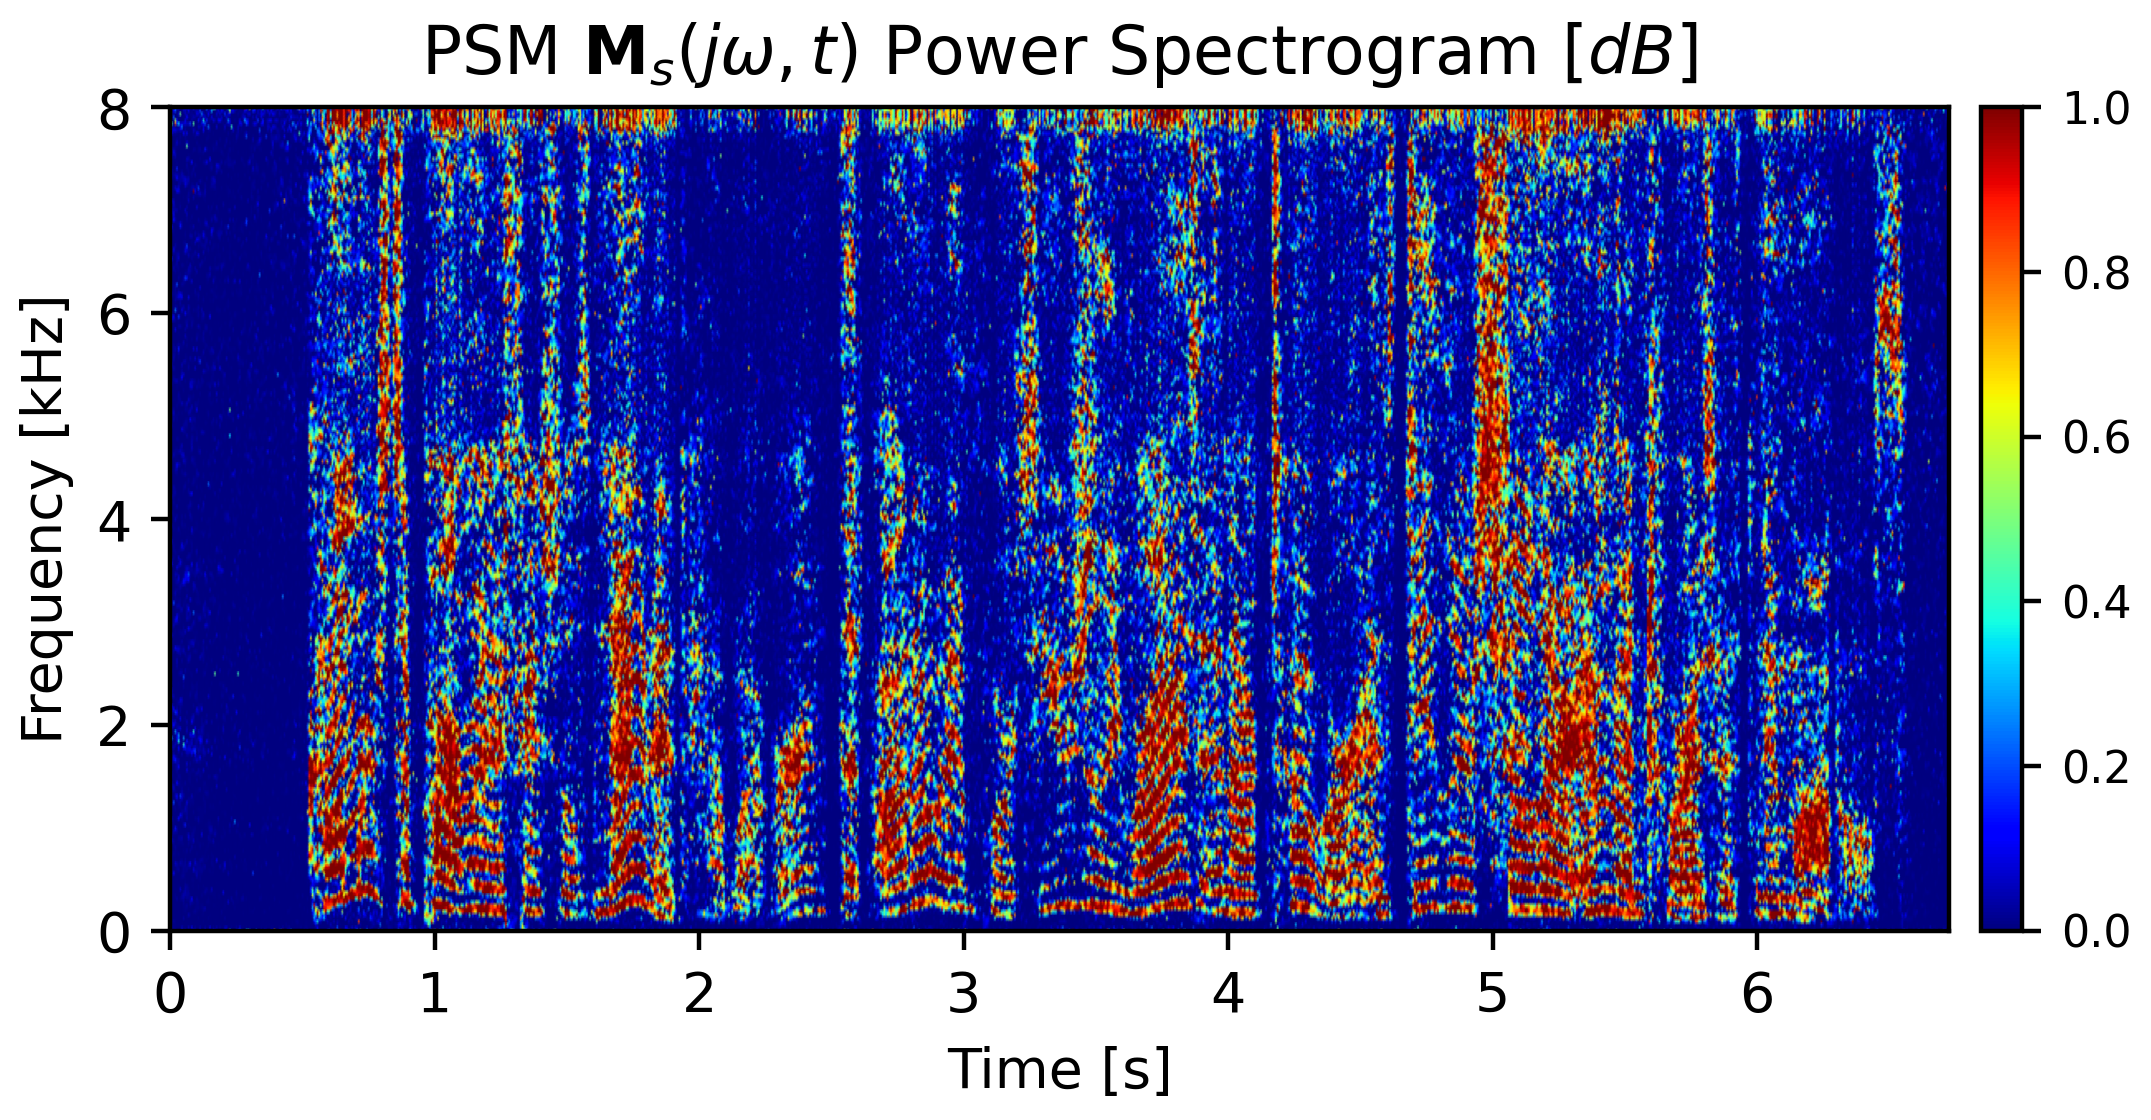
\includegraphics[width=\linewidth]{Features/images/psm_mask}
    \caption{PSM Speech Mask \(\mathbf{M}_{s}(j\omega, t)\)}\label{fig:psm_mask}
\end{figure}
\vspace{-0.5cm}
\begin{figure}[H]
    \centering
    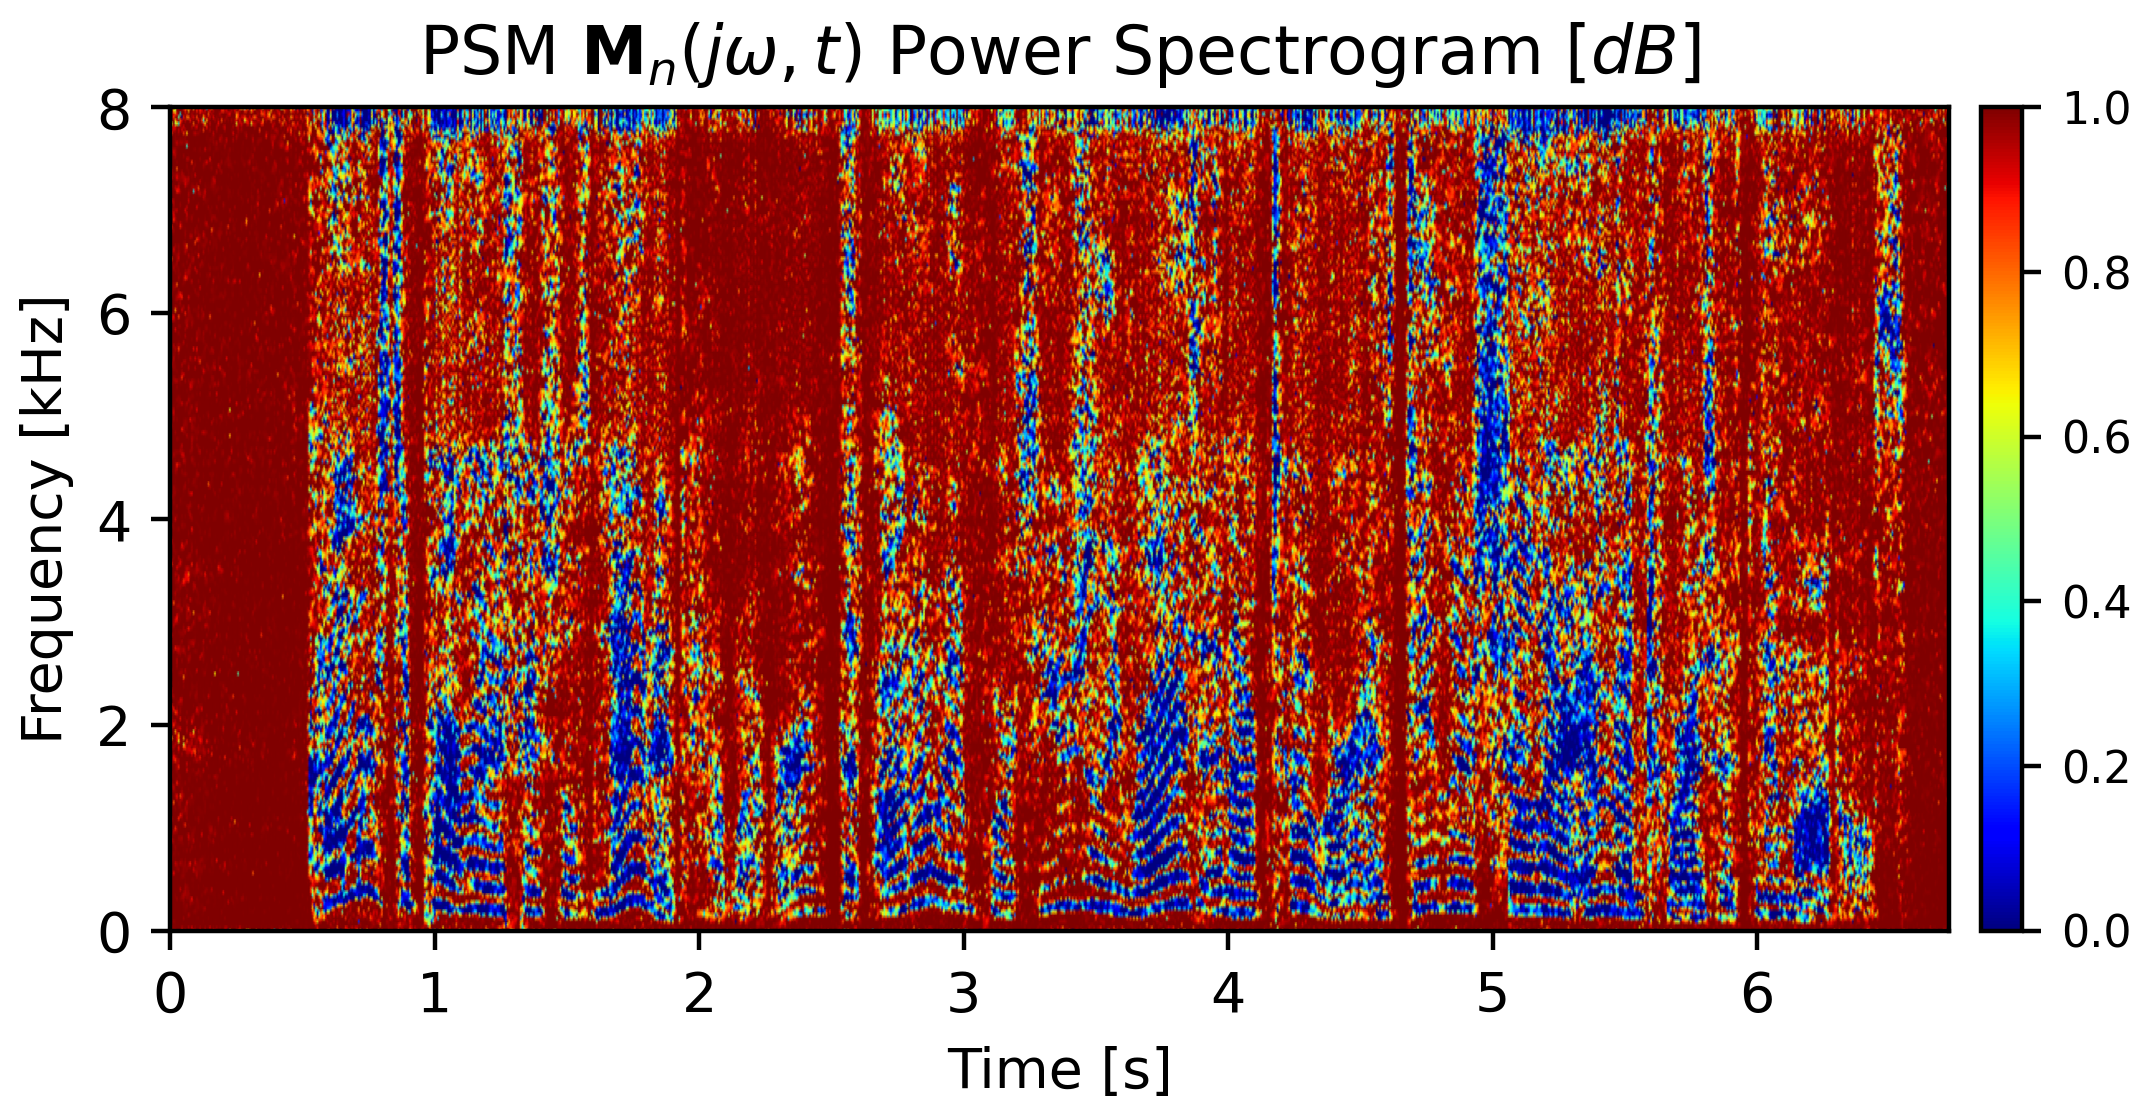
\includegraphics[width=\linewidth]{Features/images/psm_mask_noise}
    \caption{PSM Noise Mask \(\mathbf{M}_{n}(j\omega, t)\)}\label{fig:psm_mask_noise}
\end{figure}
The following equations give the PSM masks for the reference speech and noise,
\(\mathbf{M}^{(s)}_{j\omega, t}\) and \(\mathbf{M}^{(n)}_{j\omega, t}\):
\begin{align}
    \mathbf{M}^{(s)}_{j\omega, t} & = \frac{|\mathbf{S}(t,j\omega)|}{|\mathbf{Y}(t,j\omega)|} \cos(\bm{\theta}_{_{\mathbf{S}}} - \bm{\theta}_{_{\mathbf{Y}}}) \\
    \mathbf{M}^{(n)}_{j\omega, t} & = \frac{|\mathbf{N}(t,j\omega)|}{|\mathbf{Y}(t,j\omega)|} \cos(\bm{\theta}_{_{\mathbf{N}}} - \bm{\theta}_{_{\mathbf{Y}}})
\end{align}

\subsection{Masks Estimations}
Unlike the cIRM complex masks, the PSM masks are real valued.
However, the masks are not bounded similarly to the cIRM masks.
Therefore, the proposed model for the cIRM masks can be reused
with a slight difference in implementation. 
Now, only two outputs are created 
instead of branching to four outputs at the final layer.
One output for the speech mask and the other for the noise mask. 
The same as we did for the ``IRM'' but without the Sigmoids.
In addition, to deal with the unbounded range of values, 
we also apply apply a compression algorithm to the reference masks as well.
The compression mechanism is the same as 
described in Equation\;\ref{eq:cirm_compress}.

Following this architecture, the cost function can be set
to take two masks in the calculation of the error term,
like with the ``IRM'' masks:
\begin{align}\label{eq:psm_costf}
    \ell(\mathbf{\widehat{M}}_{j\omega, t},\;\mathbf{M}_{j\omega, t}) & = 
        \frac{1}{2N}\sum_{j\omega, t}
        \left[ 
            \beta\!\left( 
                \mathbf{\widehat{M}}^{(s)}_{j\omega, t} - 
                \mathbf{M}^{(s)}_{j\omega, t} 
            \right)^{2} 
            + \left( 1- \beta \right)\!
            \left(
                \mathbf{\widehat{M}}^{(n)}_{j\omega, t} - 
                \mathbf{M}^{(n)}_{j\omega, t} 
            \right)^{2} 
        \right]
\end{align}

The proposed PSM estimation network blocks diagram is shown in 
Figure\;\ref{fig:psm_nn}.

\begin{figure}[H]
    \centering
    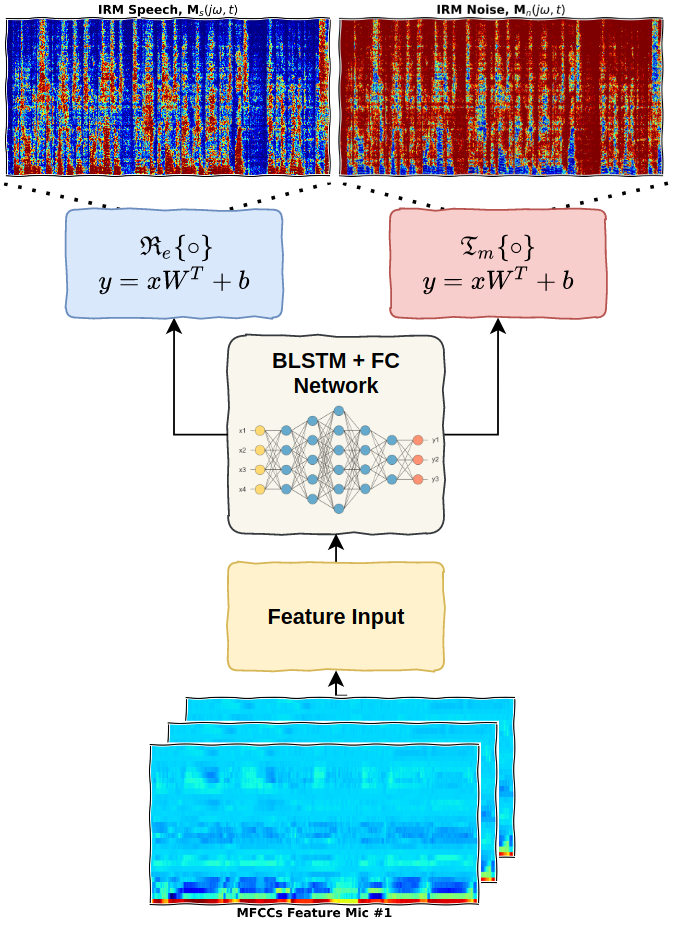
\includegraphics[width=0.75\linewidth]{Beamformers/images/psm_nn}
    \caption{Proposed DNN for PSM T-F masking estimations.}\label{fig:psm_nn}
\end{figure}

\subsection{Measurements}
\begin{figure}[H]
    \centering
    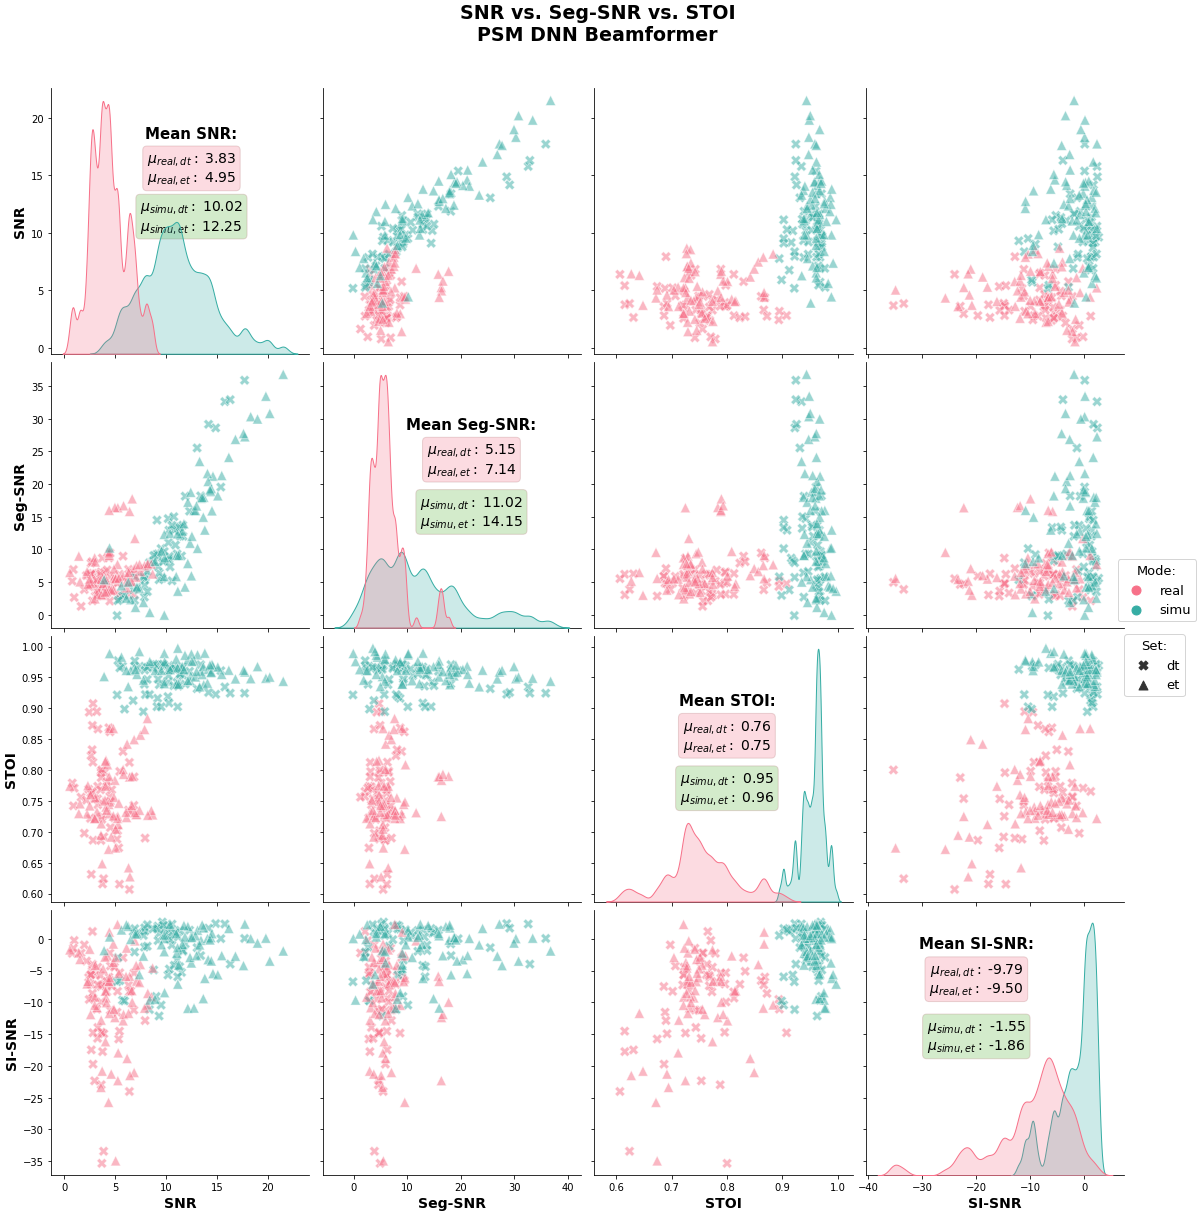
\includegraphics[width=\linewidth]{Features/images/psm_snr_stoi}
    \caption{PSM beamformer SNR vs. Segmental-SNR vs. STOI vs. SI-SNR.}\label{fig:psm_snr_stoi}
\end{figure}

\begin{figure}[H]
    \centering
    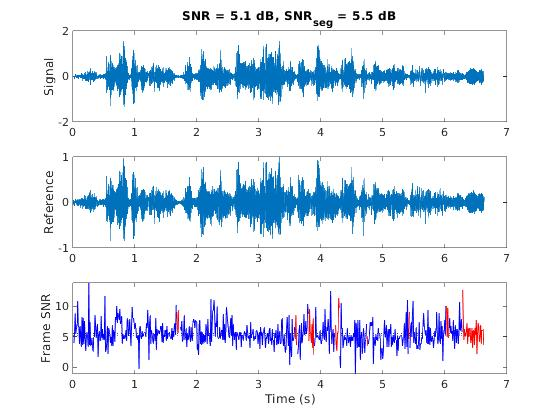
\includegraphics[width=\linewidth]{Features/images/psm_ideal_snr}
    \caption{Ideal PSM beamformer enhancement SNR \& Segmental-SNR.}\label{fig:psm_ideal_snr}
\end{figure}



\section{ORM --- Optimal Ratio Mask}
The realization of the phase component importance along with 
the desire to keep the masking as simple as possible in terms of number 
of matrices and the simplicity of multiplication for separation,
the IRM masking is further developed.

Trying to minimize the general MSE loss function for T-F masking,
same as with the ``Weiner filter'' that the IRM masking approximates, we get:
\begin{align}
    \mathbf{M}^{(s)}_{j\omega, t} & = \frac{
        |\mathbf{S}(t,j\omega)|^{2}
        + \mathfrak{R}_{e}\{ \mathbf{S}(t,j\omega) \cdot {\mathbf{N}}^{*}(t,j\omega) \}
        }{
            |\mathbf{S}(t,j\omega)|^{2} 
            + |\mathbf{N}(t,j\omega)|^{2}
            + 2 \mathfrak{R}_{e}\{ \mathbf{S}(t,j\omega) \cdot {\mathbf{N}}^{*}(t,j\omega) \} 
        } \\
    \mathbf{M}^{(n)}_{j\omega, t} & = \frac{
        |\mathbf{N}(t,j\omega)|^{2}
        + \mathfrak{R}_{e}\{ \mathbf{N}(t,j\omega) \cdot {\mathbf{S}}^{*}(t,j\omega) \}
        }{
            |\mathbf{S}(t,j\omega)|^{2} 
            + |\mathbf{N}(t,j\omega)|^{2}
            + 2 \mathfrak{R}_{e}\{ \mathbf{N}(t,j\omega) \cdot {\mathbf{S}}^{*}(t,j\omega) \} 
        }
\end{align}

Looking at the equation above, 
it resembles the IRM form but also introduces
the real part of the multiplication between the speech spectrum
and the conjugate noise spectrum.

\subsection{Masks Estimations}
The ORM masking in terms of the estimation process resembles the
PSM completely. Therefore, the same compression and 
DNN architecture are used to estimate the ORM masks.

The proposed DNN model blocks diagram is shown in Figure\;\ref{fig:psm_nn},
and the cost function is given in Equation\;\ref{eq:psm_costf}.

\subsection{Measurements}

\begin{figure}[H]
    \centering
    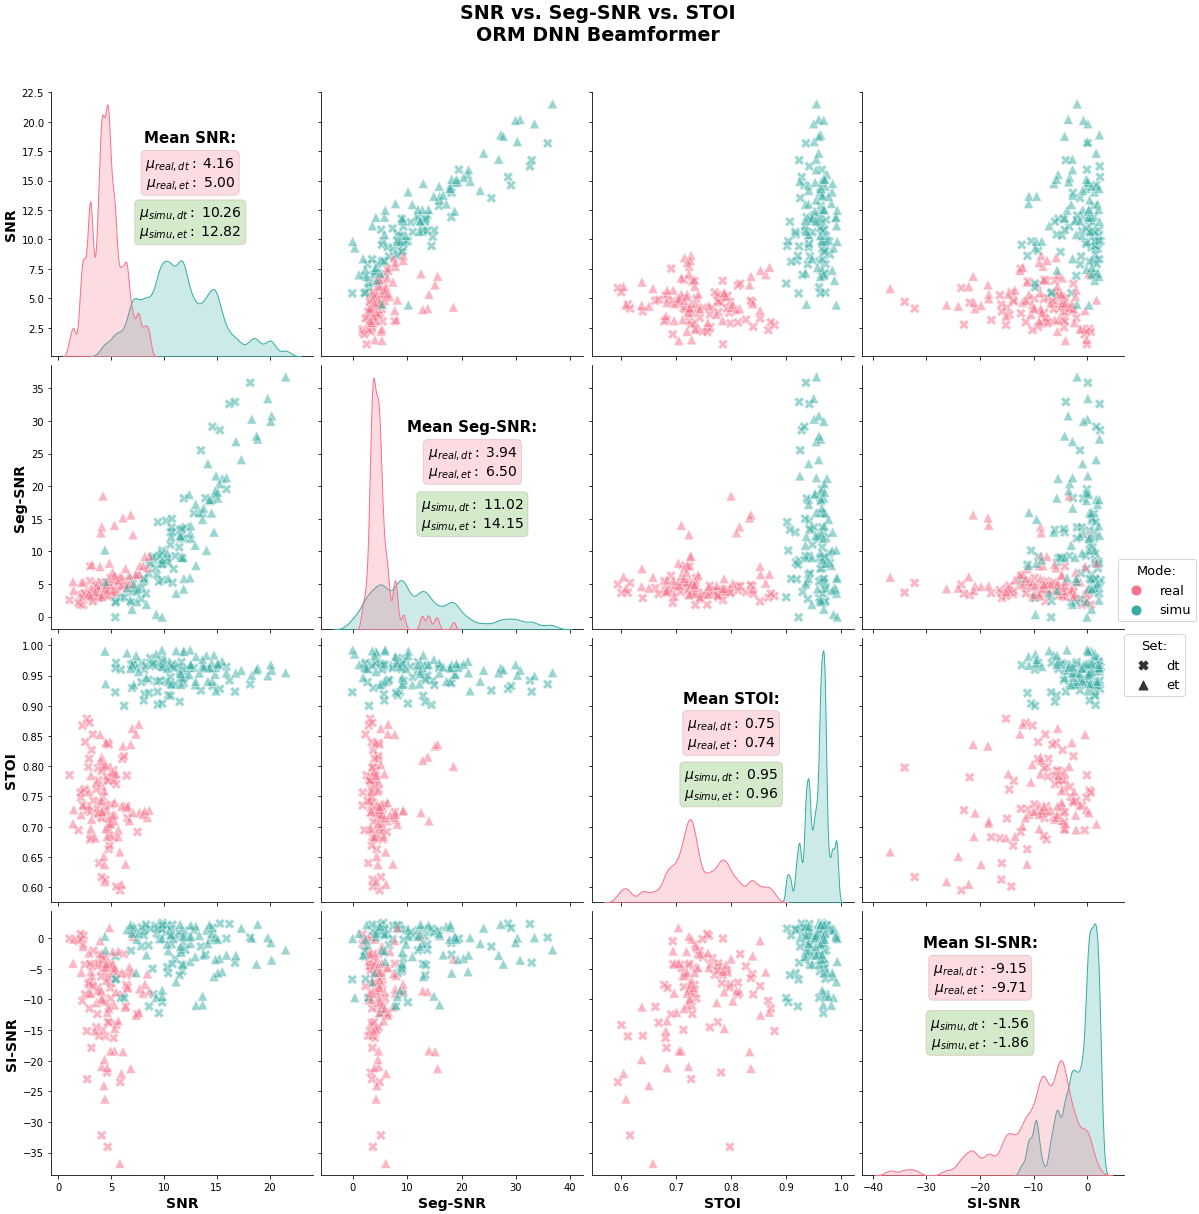
\includegraphics[width=\linewidth]{Features/images/orm_snr_stoi}
    \caption{ORM beamformer SNR vs. Segmental-SNR vs. STOI vs. SI-SNR.}\label{fig:orm_snr_stoi}
\end{figure}

\begin{figure}[H]
    \centering
    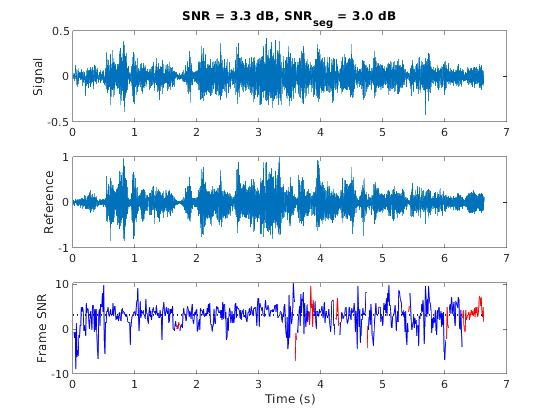
\includegraphics[width=\linewidth]{Features/images/orm_ideal_snr}
    \caption{Ideal ORM beamformer enhancement SNR \& Segmental-SNR.}\label{fig:orm_ideal_snr}
\end{figure}

% \section{Masks Estimations}
% \subsection{IRM}

% \begin{align}
%     \ell(\mathbf{\widehat{M}}_{j\omega, t},\;\mathbf{M}_{j\omega, t}) & = 
%         \frac{1}{2N}\sum_{j\omega, t}
%         \left[ 
%             \beta\!\left( 
%                 \mathbf{\widehat{M}}^{(s)}_{j\omega, t} - 
%                 \mathbf{M}^{(s)}_{j\omega, t} 
%             \right)^{2} 
%             + \left( 1- \beta \right)\!
%             \left(
%                 \mathbf{\widehat{M}}^{(n)}_{j\omega, t} - 
%                 \mathbf{M}^{(n)}_{j\omega, t} 
%             \right)^{2} 
%         \right]
% \end{align}

% \begin{figure}[H]
%     \centering
%     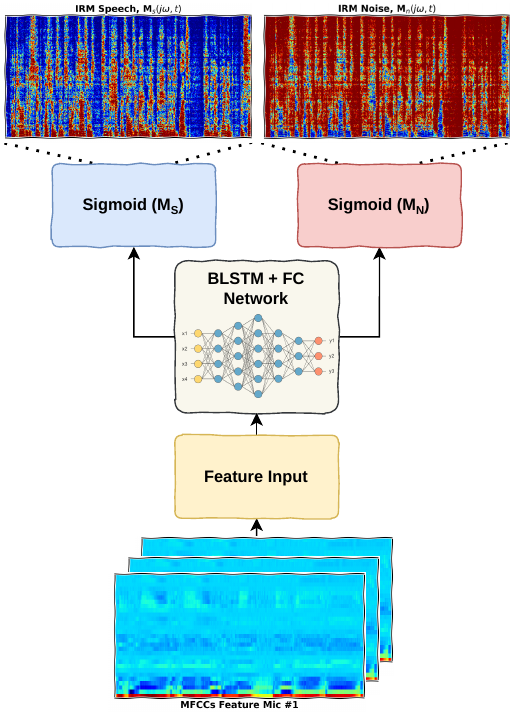
\includegraphics[width=0.75\linewidth]{Beamformers/images/irm_nn}
%     \caption{Proposed DNN for IRM T-F masking estimations}\label{fig:irm_nn}
% \end{figure}

% \subsection{cIRM}
% In Section~\ref{ssec:cirm}, 
% the \(cIRM\) masks are described in 
% Equations~\ref{eq:cirmr_mask},~\ref{eq:cirmi_mask}.
% In contrast to the \(IRM\) masks which are bounded in the range \([0, 1]\),
% the \(cIRM\) masks are unbounded, and have the range \((-\infty, \infty)\).

% A neural network cannot train for unbounded values. 
% Hence, an alternative presentation to the mask values is needed.
% One possibility is to compress the real and imaginary masks
% with a hyperbolic tangent as suggested in \cite{}: 
% \begin{align}
%     cIRM_{x} &= K \frac{1-e^{-C\cdot M_{x}}}{1+e^{-C\cdot M_{x}}}
% \end{align}

% Where \(x\), stands for the real or the imaginary parts of the mask.
% By applying this compression, the mask values are bounded in
% the range \([-K, K]\), while \(C\) controls the steepness.
% In that way, a linear layer at the output is placed
% in favor of the sigmoid layers used in the simpler IRM DNN.

% Then, the cost function is defined to include both real and imaginary parts
% of both the noise and speech masks. 
% \begin{align}
%     \ell(\mathbf{\widehat{M}}^{(x)}_{j\omega, t},\;\mathbf{M}^{(x)}_{j\omega, t}) & = 
%         \frac{1}{2N}\sum_{j\omega, t}
%         \left[ 
%             \beta\!\left( 
%                 \mathbf{\widehat{M}}^{(s \in \mathbb{C})}_{j\omega, t} - 
%                 \mathbf{M}^{(s \in \mathbb{C})}_{j\omega, t} 
%             \right)^{2} 
%             + \left( 1- \beta \right)\!
%             \left(
%                 \mathbf{\widehat{M}}^{(n \in \mathbb{C})}_{j\omega, t} - 
%                 \mathbf{M}^{(n \in \mathbb{C})}_{j\omega, t} 
%             \right)^{2} 
%         \right]
% \end{align}

% \begin{figure}[H]
%     \centering
%     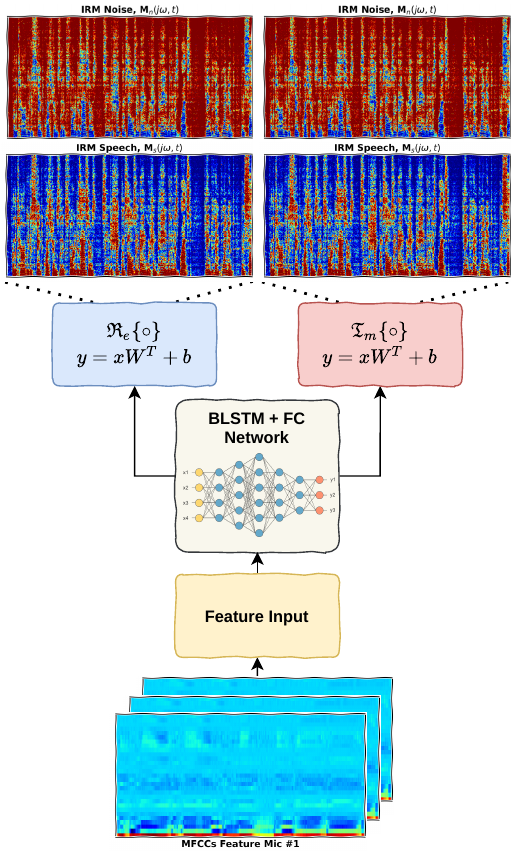
\includegraphics[width=0.75\linewidth]{Beamformers/images/cirm_nn}
%     \caption{Proposed DNN for cIRM T-F masking estimations}\label{fig:cirm_nn}
% \end{figure}


% \subsection{PSM}

% \subsection{ORM}

\section{Conclusions}
In Table\;\ref{tbl:masks_l_params} are presented
the model's sizes in terms of memory requirement
and the number of learnable parameters.
The model's parameters were quantized
to the form of signed 16 bits. 
The MSB (most significant bit) is for the sign,
the following four bits are set for the integer part,
and the other eleven bits present the fractional part.
All of the tested models were trained with and without
the \(\Delta, \Delta\Delta\) features.
Usage of the additional \(\Delta, \Delta\Delta\) features
enlarges the input size of the model and thus
leading to a larger number of learnable parameters, resulting
in a bigger model. Bigger models take a longer time to train
and are more complex to fit in limited resources hardware 
devices. A trade-off decision can be made with respect to
the memory size and desired performance in the design phase
of T-F masks based applications. Although presenting
better results in audio metrics, the PSM and ORM
masks require \(\sim 43\%\) larger memory space
compared to the IRM masks, 
when the feature set does not include
the \(\Delta, \Delta\Delta\) features.
A less severe increase of \(\sim 22\%\) in memory 
size requirement has been observed 
when the \(\Delta, \Delta\Delta\) features
were not excluded from the feature set.




\begin{table}[H]
    % for more info see: https://www.overleaf.com/learn/latex/tables
    \centering
    % \hspace*{-2.8cm}
    \arrayrulecolor{mtblborder}
\begin{tabular}{ !{\color{mtblborder}\vrule}c!{\color{mtblborder}\vrule}cc|||cc| } 
    \hline

    \hline
    \rowcolor{mtblcaption}
    & \multicolumn{2}{c}{\color{white}\bf{Learnable Parameters} [Mil]}
    & \multicolumn{2}{c}{\color{white}\bf{Quant. (S16.11) Mem } [Mb]}\\         
    % \cline{2-8}
    
    \multirow{-2}{*}{\cellcolor{mtblcaption}\color{white}\bf{Targets} }
    & \cellcolor{mtbl} \color{black}{W/o (\(\Delta\),\(\Delta\Delta\))} 
    & \cellcolor{mtbl} \color{black}{W/ (\(\Delta\),\(\Delta\Delta\))}
    & \cellcolor{mtbl} \color{black}{W/o (\(\Delta\),\(\Delta\Delta\))} 
    & \cellcolor{mtbl} \color{black}{W/ (\(\Delta\),\(\Delta\Delta\))} \\
    % & \color{white}\bf{ORM} 
    % & \color{white}\bf{Clean} \\
    \hline

    \hline
    \rowcolor{mtblA} IRM  
        & 2.44 
        & 4.67
        & 39.0
        & 74.8 \\
    \hline
    
    \hline
    \rowcolor{mtbl} cIRM  
        & 3.76
        & 5.99
        & 60.1
        & 95.9 \\
    \hline

    \hline
    \rowcolor{mtblA} PSM  
        & 3.49
        & 5.73
        & 55.9
        & 91.7 \\
    \hline

    \hline
    \rowcolor{mtbl} ORM  
        & 3.50
        & 5.74
        & 56.0
        & 91.8 \\
    \hline
    
    \hline
\end{tabular}
\arrayrulecolor{black}
\caption{T-F Masks models learnable parameters vs. Required memory size}
\label{tbl:masks_l_params}
\end{table}